\documentclass[10pt, twoside]{article}

\RequirePackage{amsmath}
\RequirePackage{amsthm}
\RequirePackage{amssymb}
% \RequirePackage[top=2cm, asymmetric, left=2.5cm, right=6cm]{geometry}
\RequirePackage[top=2cm, inner=2.5cm, outer=6cm]{geometry}

\RequirePackage{titlesec}
\RequirePackage[hidelinks]{hyperref}
\RequirePackage[english]{babel}
\RequirePackage[autostyle, english=american]{csquotes}
\RequirePackage[skip=8pt]{parskip}
\RequirePackage{caption}
\RequirePackage[nodisplayskipstretch]{setspace}
\RequirePackage{mathtools}
\RequirePackage{xcolor}
\RequirePackage{colortbl}
\RequirePackage{tcolorbox}
\RequirePackage{enumitem}
\RequirePackage{multicol}
\RequirePackage{subcaption}
\RequirePackage{ifthen}
\RequirePackage{MnSymbol}
\RequirePackage{algpseudocode}
\RequirePackage{mathrsfs}
% \RequirePackage{mleftright}
% \mleftright
\RequirePackage{tikz}
\RequirePackage{tikz-3dplot}
\RequirePackage{tikzscale}

\usetikzlibrary{tikzmark}
\usetikzlibrary{calc}
\usetikzlibrary{decorations.pathmorphing}
% \usetikzlibrary{3d}

% While I think Libertine looks the best out of the fonts I've tried, I still
% feel like I can find a better combination of fonts, so I've been trying a few.
% It turns out that dealing with fonts in latex (well pdflatex at least) can be
% quite the headache sometimes. Inconsolata is pretty much set for the
% monospace font though.

% \RequirePackage{cmbright}
% \usepackage[t,lf]{spectral}

\RequirePackage{libertine}
\RequirePackage{libertinust1math}

% \RequirePackage[default,regular,semibold,scale=0.9]{sourceserifpro}

% Garamond seems to be quite the quite the pain to get working (especially to
% get a decent looking font weight). The medium weight font looks nice except
% for some reason it only seems to appear in amsthm environments and not in the
% global text, which is puzzling and slightly annoying. Also, ebgaramond-maths
% overrides any options you send to ebgaramond. If one tries to send these
% options to ebgaramond-maths, they don't work so uhhhhhh the package is kinda
% useless in that regard. Oldstyle numbers look pretty bad, which is why it's a
% dealbreaker.
% \usepackage[T1]{fontenc}
% \usepackage[m, sb, lf]{ebgaramond}

\RequirePackage{inconsolata}

\MakeOuterQuote{"}

% Paragraph styling
\setlength{\parindent}{0pt}
\renewcommand{\baselinestretch}{1.0}

% Section customizing
\titleformat{\section}[hang]{\LARGE}{}{0pt}{}[{\titlerule[0.5pt]}]
\titleformat{\subsection}{\bfseries}{}{0pt}{}

%\titlespacing{\section}{-20pt}{20pt}{10pt}
\titlespacing{\section}{0pt}{20pt}{10pt}

\definecolor{fadegray}{RGB}{160, 180, 180}

\newcommand{\NewSection}[2]{\section{#1\hfill\color{fadegray}#2}}

\newcommand{\MarginComment}[1]{\marginpar{\fontsize{8pt}{10pt}\selectfont #1}}

\DeclareCaptionFormat{custom}{
    \textbf{#1.} #3
}

\captionsetup{
    font=footnotesize,
    format=custom
}

\newtcolorbox{blackbox}{colback=white, boxrule=0.7pt, colframe=black, sharp corners}

\theoremstyle{definition}
\newtheorem*{problem}{Problem}

\widowpenalties 1 10000

\setlength{\abovedisplayskip}{-15pt}
\setlength{\belowdisplayskip}{0pt}
\setlength{\abovedisplayshortskip}{-15pt}
\setlength{\belowdisplayshortskip}{0pt}

\renewcommand{\qedsymbol}{\ensuremath{\blacksquare}}

\setlist[enumerate, 1]{label=\textbf{\arabic*.}}

\usetikzlibrary{positioning}

\newcommand{\set}[1]{\ensuremath{\left\{ #1 \right\}}}

\newcommand{\bvec}[1]{\ensuremath{\mathbf{#1}}}
\newcommand{\conj}[1]{\ensuremath{\overline{#1}}}
\newcommand{\abs}[1]{\ensuremath{\left\lvert #1 \right\rvert}}
\newcommand{\floor}[1]{\ensuremath{\left\lfloor #1 \right\rfloor}}
\newcommand{\bounds}[3]{\ensuremath{\left. \rule{0pt}{10pt} #1 \: \right\vert_{#2}^{#3}}}

% Log denoting the principal branch of the complex logarithm
\DeclareMathOperator{\Log}{Log}
\DeclareMathOperator{\Arg}{Arg}

% Why aren't these defaulty defined? No love for the other inverse trig
% functions u_u
\DeclareMathOperator{\arcsec}{arcsec}
\DeclareMathOperator{\arccot}{arccot}
\DeclareMathOperator{\arccsc}{arccsc}

% It seems these are already defined
% Not really sure whether standard serif is better than frakture but we'll see.
% \DeclareMathOperator{\Re}{\mathfrak{Re}}
% \DeclareMathOperator{\Im}{\mathfrak{Im}}

\DeclareMathOperator{\LaplaceL}{\mathscr{L}}
\DeclareMathOperator{\InvLaplaceL}{\mathscr{L}^{-1}}
\newcommand{\Laplace}[1]{\ensuremath{\LaplaceL \left\{ #1 \right\} \left( s \right)}}
\newcommand{\InvLaplace}[1]{\ensuremath{\InvLaplaceL \left\{ #1 \right\} \left( t \right)}}

\DeclareMathOperator{\Heaviside}{H}
\DeclareMathOperator{\Rect}{\Pi}


\title{The Math Journal}
\author{Rushil Surti}

\begin{document}

% Title Page
\begin{titlepage}
\newgeometry{}

\maketitle

\restoregeometry
\end{titlepage}

\newpage

\tableofcontents

\newpage
% We will organize the entries in the filesystem as such
% - main.tex
% - entries
%   - entry000
%     - index.tex
%     - body.tex
%   - entry001
%     - index.tex
%     - body.tex
%   - ...

% index.tex will contain some of the parts that should be
% separated from the writing view, such as the section
% header and potentially small section table of contents.
% The actual writing will be placed in body.tex, which is
% included by index.tex for convenience.

% Aside: Why use numbers to identify the entry instead of a short
% description of what it's about?
% While it might help when searching in files to have a short title
% as the filename instead of some arbitrary number, there are a few
% complications:
% 1. (Good) names are hard to come up with.
% 2. Detailed title names lose any sort of uniformity in filenames.
%    What if I want to (for example) create a program that fills in
%    the boilerplate necessary to create a new directory (allowing me
%    to just get straight into writing)? With named titles this is hard
% As a compromise, it is trivial to simply use grep and search through
% all files to find what exactly I'm looking for. I can even put in keywords
% in the index.tex or body.tex file if needed.
\NewSection{What \textit{is} a Math Journal Anyways?}{2023-03-28}

This is hopefully going to be the start of something fun! I've been wanting a
space to document, formalize, and just have fun typesetting things and ideas
that I've been working on relating to (mostly) math. \MarginComment{This is
also very much a testing ground for my \LaTeX\ styling stuff, so keep that in
mind ;)} This journal will probably contain everything that goes into that
process: my musings, results, and work, although I'll try and keep the actual
line-for-line scratch work to a minimum, because that looks bad and isn't very
helpful. Who knows, I'll probably even throw in a couple contest math problems!

All in all, I intend to go back to previous results that I've worked on as well
as anything I come up with. This may result in a lot of sections that will be
"TODO," but I guess you can't finish all your side projects, right?

As you can probably tell, the tone is going to be quite conversational and
decently informal, but I'm not going to jump into "zoomer language" and meme
around \textit{too much}. That being said this is all for fun.

\MarginComment{
    \begin{center}
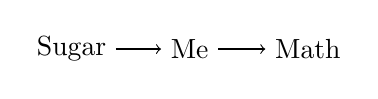
\begin{tikzpicture}
    \draw (-1.5, 0) node (sugar) {Sugar};
    \draw (0, 0) node (me) {Me};
    \draw (1.5, 0) node (math) {Math};

    \draw[->] (sugar) -- (me);
    \draw[->] (me) -- (math);
\end{tikzpicture}
\end{center}

    \captionof{figure}{My daily schedule}
}

One might also ask the question, why are you writing this as if someone will
read it when in all likelihood it won't be read much? To that hypothetical
question posed by myself to myself about writing to myself, I must answer that
this is far too philosophical for me and we must move on. It's math time!


\NewSection{Covering the Cartesian Coordinates}{2023-03-29}

Whoo boy after some brief styling with the document, it's finally time to get
to our very first entry! This problem really isn't anything amazingly special
to commemorate the occasion or anything, though; it's just the first one I had
on hand.

After drudging through the \( n \)th tangent line problem for the AP review, I
\MarginComment{Even I sometimes come up with some interesting stuff, right?
\textit{Right}?} started to get bored and my mind drifted. This is when I
thought of the following problem.

\begin{blackbox}
    \begin{problem}
        Let \( T \) denote the set of all points contained within every line
        tangent to some function \( f \left( x \right) \). Is there a function
        \( f \left( x \right) \) such that \( T = \mathbb{R}^2 \)?
    \end{problem}
\end{blackbox}

This problem evolved after thinking about it for a while and actually trying
\MarginComment{And I also like doing this because it details my thinking
process and also simply goes to show that no mathematician is truly
perfect. Math is a journey and behind every proof or problem there's
potentially a lot of trial and error that happens, so don't be discouraged!}
things out, but I thought I would at least share the original problem and my
thoughts on it.

\subsection{Playing Around with the Idea}

I'm sure there's a lot of ways to start to tackle a problem like this, and
depending on your experience, you may or may not quickly find something to
latch onto, but one of the tried and true things to do is just play around with
the problem. What exactly are we asking for, and what sort of assumptions can
we make to narrow down the scope of the problem?

\begin{figure}[ht]
    \centering
    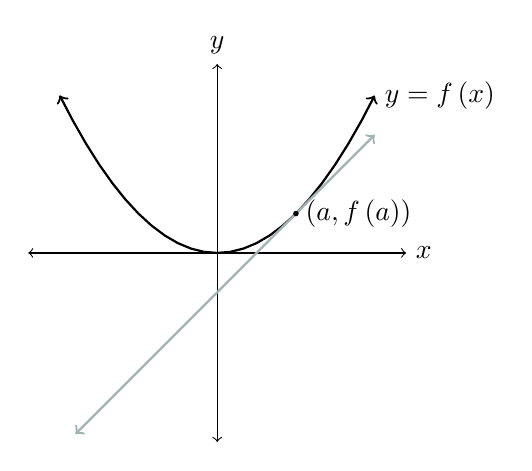
\begin{tikzpicture}[domain=-1:1, scale=2]
    \draw[<->] (-1.2, 0) -- (1.2, 0) node[right] {\( x \)};
    \draw[<->] (0, -1.2) -- (0, 1.2) node[above] {\( y \)};

    \draw[<->, thick] plot (\x, \x * \x) node[right] {\( y = f \left( x \right) \)};
    
    \draw[<->, fadegray, thick] (-0.9, -0.9 - 0.25) -- (1, 1 - 0.25);
    \fill (0.5, 0.25) circle[radius=0.5pt] node[right] {\( \left( a, f \left( a \right) \right) \)};
\end{tikzpicture}

    \captionof{figure}{Imagine dragging a point with its tangent line along some function \( f \left( x \right) \).}
\end{figure}

First, let's get a visual intuition for what we're actually measuring. Imagine
for some function \( f \left( x \right) \) dragging a point along the curve and
looking at the tangent line at that curve. For some curves, this tangent line
will stay relatively similar (especially for functions with a constant
derivative, which should make sense); however, for other functions, this
tangent line will "sweep" across the plane, which is the ideal behavior we're
looking for.

Now \MarginComment{Remember, even if these don't mean much, that's fine! All
we're trying to do is empty our brains and think of something that will lead us
to a potential solution.} the problem has reduced to finding a function that
will sweep through the \textit{entire} Cartesian plane. This corresponds to a
function whose derivative has the following properties:

\begin{enumerate}
    \item A change in sign. If the derivative is always positive or always
    negative, there's going to be some part of the plane that the tangent
    lines will never reach, so the sign must flip somewhere.
    \item Some sort of periodicity. Coupled with a change in sign, if we can
    have the derivative be periodic in some form, it may reduce down to
    some repeatable pattern covering the plane.
    \item Steep lines. Perhaps subjective and not necessarily a requirement,
    but derivatives with high magnitude will likely reach more points.
\end{enumerate}

Keeping this in mind, let's explore and essentially just guess some possible
solutions. If we think about it for a minute though, we can actually come up
with quite a few solutions! Right off the bat, we can see \( f \left( x \right)
= \sin{\left( x \right)} \) is a applicable solution. So long as we keep on
moving to infinity, the tangent line will keep sweeping through the plane.

One could try and make the argument for a function defined over a finite
domain, but this is easily adjustable with a simple change of argument such as
\( f \left( x \right) = \sin{\left( 1/x \right)} \) or \( f \left( x \right) =
\sin{\left( \ln{\left( x \right)} - \ln{\left( 1 - x \right)} \right)} \), both
of which compress the entire domain of our wave into a finite domain. In fact,
a far more challenging (and interesting) problem to tackle would be finding a
function such that \( T = \mathbb{R}^2 \setminus P \), with \( P \) being some point
on the Cartesian plane. In order to do this, however, we must introduce some
some of quantitative metric to find out whether a point truly is included in \( T \).

\subsection{Doing the Math\texttrademark}

Now that we've looked at some intuition for what's happening and realized that
we would like to make some adjustments to the problem, it's time to actually
get down to business and figure out how to determine whether a point is in our
set \( T \).

\begin{proof}
Given \MarginComment{I'm no expert on proofs and rigour (but I'm trying my best to improve!) so some of my arguments may be lacking in areas throughout this entire journal. But you'll forgive me, right? :)} some point \( a \) on \( f \left( x \right) \), we have the following line tangent to the function:
\[
    L_a \left( x \right) = f' \left( a \right) \left( x - a \right) + f \left( a \right)
.\]
In order for some point \( P \) to be contained in this tangent line, we must
set \( x \) to \( P_x \) \MarginComment{I'm using "vector" notation for the
    components of these points because its far more convenient that way. For
    anyone unfamiliar, we take \( P_x \) to denote the \( x \) part of the
point \( P \) and similarly \( P_y \) represents the \( y \) part of \( P \)}
and \( L_a \left( x \right) \) to \( P_y \). This will then give us some
function in \( a \), which tells us something about whether \( P \) is in \( T
\). If there exists an \( a \) which solves the equation, we know that the
point must be included in the set of points that the tangent lines contain. If
not, however, we can say for certain that this point is not in \( T \).

We can use this strategy to now show that \( f \left( x \right) = \sin{\left( x
\right)} \) covers the entire Cartesian plane. Let us test any point \( P \)
using the previous equation.
\[
    P \in T \iff 0 = \cos{\left( a \right)} \left( P_x - a \right) + \sin{\left( a \right)} - P_y
.\]
In cases like this, it is far easier to tools from calculus to verify that a
solution exists rather than solving for it explicitly. Let us call the right
hand side of our modified linearization "discriminant" function \MarginComment{I wasn't really sure what to call it so I landed on discriminant function. A "discriminating" function doesn't sound very nice now does it? :)} \( \phi_P \left( a \right) \),
where \( P \) represents the point we are testing. If we
vary \( a \), we see the following holds true.
\begin{align*}
    & \lim_{a \to \infty} \phi_P \left( 2 \pi a \right) \to -\infty \\
    & \lim_{a \to -\infty} \phi_P \left( 2 \pi a \right) \to \infty
.\end{align*}
It is trivial to see then by the Intermediate Value Theorem that there exists
some value of \( a \) on the number line in which \( \phi_P \left( a \right) = 0 \), which means
that there exists some solution to our discriminant equation. Due to this applying
for any arbitrary point \( P \), we have just shown that the entire Cartesian plane is
contained in \( T \) for \( f \left( x \right) = \sin{\left( x \right)} \).
\end{proof}

Now that we have verified and familiarized ourselves with some of the tools at
use here, let's go back to our modified problem. Can we construct a function
where all but \textit{one single point} in the Cartesian plane is included in \( T \)?

\subsection{The Modified Problem}

This problem is a bit harder to tackle, especially at first glance. In the end,
this boils down to whether or not we can find a function with some specific
characteristics.

% Change all the points with (x1, y1) to Q_x and Q_y because idk it feels
% better than just randomly having x and y values that have a subscript index
% but not having the existence of any other points.
\begin{enumerate}
    \item For every point \( Q \) that is not \( P \),
        there must exist an \( a \) value such that our condition
        \( 0 = f' \left( a \right) \left( Q_x - a \right) + f \left( a \right) - Q_y \)
        holds.
    \item Specifically for the point \( P \), there must be no solution to the given the preceding condition.
\end{enumerate}

Just to simplify things a little bit, let's take \( P \) to be the point
\( \left( 0, 0 \right) \) and see what happens. Concretely, let's take a look at
the second condition, as it seems much stronger (and thus can narrow down our
choice of \( f \), if any). The condition now becomes that there must be
\textbf{no} value of \( a \) such that the following has as solution:
\[
    0 = -a f' \left( a \right) + f \left( a \right) = \phi_P \left( a \right)
.\]
Utilizing this and the fact that \( f \) is continuous, we can split this into two (likely symmetric) cases.
\begin{multicols}{2}
\begin{enumerate}
    \item \( \phi_P \left( a \right) > 0 \) for all \( a \)
    \item \( \phi_P \left( a \right) < 0 \) for all \( a \).
\end{enumerate}
\end{multicols}
We see that this must be the case once again due to the Intermediate Value
Theorem. This also shows that the condition that \( f \) must be continuous
over all real numbers is quite limiting.

Let us suppose we have some function \( f \) where the first case is true.
Notice then that if we let \( Q \) be of the form \( \left( P_x, y \right) = \left( 0, y \right) \) for some arbitrary \( y \), something quite interesting happens. Let us examine our discriminant functions again.
\begin{align*}
    \phi_P \left( a \right) &= -a f' \left( a \right) + f \left( a \right) \\
    \phi_Q \left( a \right) &= -a f' \left( a \right) + f \left( a \right) - y = \phi_P \left( a \right) - y
\end{align*}
Notice that when we pick a point directly above or below \( P \), it
corresponds to simply vertically shifting \( \phi_Q \left( a \right) \).
Keeping in mind that we want \( \phi_P \left( a \right) \) to \textit{never}
have a solution and \( \phi_Q \left( a \right) \) to \textit{always} have a
solution, this poses a complication.

With this, supposing that \( \phi_P \left( a \right) \) is always greater than
\( 0 \), there will always be a sufficiently large negative \( Q_y \) value
such that \( \phi_Q \left( a \right) \) does not have a solution. Vice versa, a
similar condition holds for when \( \phi_P \left( a \right) \) is always less
than \( 0 \). Thus, there exists \textbf{no continuous function \( f \) of \( x
\) such that all but one point is included in the set of points of its tangent
lines.} Truly a shame, but its cool that we can prove this.

To offer a visual intuition for why this is the case, consider the function \(
f \left( x \right) = 1/x^2 \). \MarginComment{This choice isn't quite continuous
over all reals, but we'll let it slide because it was chosen in order to
illustrate a point more than anything} As we head to the infinities at either side of the graph, the line gets closer and closer to obtaining a slope of \( 0 \). However, as we approach the pole at \( x = 0 \), the function quickly picks up and the line will get ever close to being vertical. This colors all of the Cartesian plane, \textit{except} for one particular strip of values on the negative \( y \)-axis.

\subsection{Remarks}

While we have shown that there exists no function of \( x \) with the
properties described in the modified problem. One should note that the solution
is almost trivial if we turn to the world of parametric functions. Consider a function \( f \) defined as such:
\begin{align*}
    f_x \left( t \right) &= \varepsilon \cos{\left( t \right)} \\
    f_y \left( t \right) &= \varepsilon \sin{\left( t \right)}
\end{align*}
If we take \( \varepsilon \to 0^+ \), we quickly see the desired behavior. The
fucntion, infinitely close to being a point, hugs the boundary of \( \left( 0,
0 \right) \), with the tangent line going through all points except \( \left(
0, 0 \right) \). If we wanted to have this centered around some arbitrary
point, all we would have to do is simply add or subtract from the respective
function components.

\subsection{Conclusion}

All in all, this was a sort of interesting problem, and I'm at least proud of
it! It wasn't all that difficult and didn't require any higher level tools
besides some calculus, but that in of itself is quite nice. I hope to find some
similarly interesting problems that apply what the classroom teaches and goes
beyond that, requiring some problem solving skills. Who knows? Maybe there's
already a competition problem or such revolving around the concept. I wouldn't
be too surprised if there was.

With that, this is the end of the first entry in this journal. Hopefully it isn't the last :)


\NewSection{General Product Rule}{2023-04-06}

We all know and love (well hopefully) the famous product rule for derivatives, given as follows:
\[
    \frac{d}{dx} \Bigl( f \left( x \right) g \left( x \right) \Bigr) = f \left( x \right) g' \left( x \right) + f' \left( x \right) g \left( x \right)
.\]
But here's an interesting question. What happens when we have more than two
\MarginComment{Finally! A problem that won't make me tear my hair out.}
functions of \( x \) multiplied together? The result is what's called the
Leibniz product rule. Let's derive it!

\begin{blackbox}
    \begin{problem}
        What does the following evaluate to?
        \[
            \frac{d}{dx} \prod_{i = 1}^{n} f_i \left( x \right)
        \]
    \end{problem}
\end{blackbox}

\subsection{Solving}

To be honest, there isn't much complicated machinery involved in this one. First, let's observe what happens we increase the number of functions.

\textit{Case} \( n = 3 \):

We want to take the derivative of the product \( f_1 \> f_2 \> f_3 \). \MarginComment{It's a bit noisy with all the \( x \) arguments, so while I'll omit them here, just know that these are all functions of \( x \).} Left with no other choice, we proceed by using our normal product rule, taking our left function to be \( f_1 \) and our right function to be the product \( f_2 \> f_3 \), resulting in the following:
\begin{align*}
    \frac{d}{dx} \Bigl( f_1 \cdot f_2 \> f_3 \Bigr) &= f_1' \> f_2 \> f_3 + f_1 \cdot \frac{d}{dx} \Bigl( f_2 \> f_3 \Bigr) \\
    &= f_1' \> f_2 \> f_3 + f_1 \cdot \left( f_2' \> f_3 + f_2 \> f_3' \right) \\
    &= f_1' \> f_2 \> f_3 + f_1 \> f_2' \> f_3 + f_1 \> f_2 \> f_3'
.\end{align*}

\textit{Case} \( n = 4 \):
One may also verify the following, using the fact that we have already found the derivative for three functions.
\[
    \frac{d}{dx} \Bigl( f_1 \> f_2 \> f_3 \> f_4 \Bigr) = f_1' \> f_2 \> f_3 \> f_4 + f_1 \> f_2' \> f_3 \> f_4 + f_1 \> f_2 \> f_3' \> f_4 + f_1 \> f_2 \> f_3 \> f_4'
.\]

It may become clear now that we have a pattern forming with a rather beautiful symmetry. It seems that when we take the derivative of the product of these \( n \) functions, it splits into \( n \) terms each with the same product except for one function's derivative being taken. This recurrence forming in the pattern may also help motivate our method of proof of this a little bit later on.

This can be expressed a little more compactedly (although perhaps less illuminatingly) as the following:
\[
    \frac{d}{dx} \prod_{i = 1}^{n} f_i \left( x \right) = \sum_{i = 1}^{n} f_i' \left( x \right) \prod_{\substack{j = 1 \\ j \ne i}}^{n} f_i \left( x \right)
\]

We shall now show this rigorously.

\begin{proof}
    We shall show this using proof by induction. For our base case, the case \( n = 1 \) or \( n = 2 \) are quite trivial.

    Next, suppose that for some \( k \) we have that
    \[
        \frac{d}{dx} \prod_{i = 1}^{k} f_i \left( x \right) = \sum_{i = 1}^{k} f_i' \left( x \right) \prod_{\substack{j = 1 \\ j \ne i}}^{k} f_i \left( x \right)
    \]
    We now must show that the same holds when we increase \( k \mapsto k + 1 \), effectively multiplying inside the derivative by a new function \( f_{k+1} \). Taking one side to be \( f_{k+1} \) and the other to be our big product, we can continue with regular product rule.
    \begin{align*}
        \frac{d}{dx} \Bigl( f_{k+1} \cdot \prod_{i = 1}^{k} f_i \left( x \right) \Bigl) &= f_{k+1} \cdot \sum_{i = 1}^{k} f_i' \left( x \right) \prod_{\substack{j = 1 \\ j \ne i}}^{k} f_i \left( x \right) + f_{k+1}' \prod_{i = 1}^{k} f_i \left( x \right) \\
        &= \sum_{i = 1}^{k} f_i' \left( x \right) \prod_{\substack{j = 1 \\ j \ne i}}^{k + 1} f_i \left( x \right) + f_{k+1}' \prod_{i = 1}^{k} f_i \left( x \right)
    \end{align*}
    With this, \MarginComment{You know, there's actually quite the bit of "symbol soup" going on here. Perhaps expanding this would make it look more reasonable? I'll have to revisit this sometime because I don't think the math nor the explanation are very helpful if you don't have the idea in mind.} we're almost where we want to be at. After bringing the \( f_{k+1} \) term inside the product on the right side, notice that we have in our left term all "groups of terms" where there is one derivative \textit{except} for \( f_{k+1} \), and on the right side, we have our \textit{only} derivative being \( f_{k+1} \). We can bring this right term inside, now giving us our desired form.
    \[
        \frac{d}{dx} \prod_{i = 1}^{k + 1} f_i \left( x \right) = \sum_{i = 1}^{k + 1} f_i' \left( x \right) \prod_{\substack{j = 1 \\ j \ne i}}^{k + 1} f_i \left( x \right)
    \]
    This concludes the proof.
\end{proof}

\subsection{Uses}
The reader may now be wondering, what could possibly be the use of such a formula? Indeed, it's not \textit{too} often that one needs to take the derivative of a large product (for a Taylor series, you'd need to be able to take \( n \) derivatives, and that gets quite hairy in of itself); however, allow me to offer at least one "cool" \MarginComment{Well at the very least, I think it's cool!} example. One of the times you may see a product that works very well for these cases is a factored polynomial.

Consider a polynomial \( P \left( x \right) \) that has \( n \) distinct \MarginComment{These roots necessarily have to be distinct, as we'll see later ;)} roots \( r_1,r_2,\ldots,r_n \). We can write the polynomial as the following:
\[
    P \left( x \right) = \prod_{i=1}^{n} \left( x - r_i \right)
.\]
Perhaps you can see where I'm going with this. Using our generalized product rule, we can take the derivative of \( P \left( x \right) \), noting that each individual term has a derivative of simply \( 1 \) due to it being a linear term.
\[
    P' \left( x \right) = \sum_{i = 1}^{n} \prod_{\substack{j = 1 \\ j \ne i}}^{n} \left( x - r_j \right)
\]
This in of itself isn't all too interesting, following directly from our generalized product rule. If we plug in \textit{the roots} into the derivative, however fun things happen with canceling. Taking \( x \) to be some arbitrary root \( r_j \), we have that
\[
    P' \left( r_j \right) = \prod_{\substack{i = 1 \\ i \ne j}}^{n} \left( r_j - r_i \right)
\]
For \textit{any polynomial}, the derivative of it at some root is the product of the differences of that root with all the others. That's pretty cool.

Remember, back to when we said that these roots have to be \textit{distinct}? If we now relax that and instead say that some root \( r_j \) has a multiplicity greater than one, something else happens instead. Because we only take the derivative of one of the terms containing \( x - r_j \), there are still other terms with this, making the derivative \( 0 \) altogether. This tells us that for any polynomial, there is going to be a horizontal tangent at any root whose multiplicity is greater than one. That's also pretty \textit{smooth} if I do say so myself.


\NewSection{Realigning Some Rotations}{2023-04-26}

Here's a cute little problem that I actually had to solve while programming a
Rubik's cube in 3D. While rotating the cube in small steps, we can keep a
matrix in the background that keeps track of these rotations applied to the
cube in case we need to invert them. \MarginComment{Specifically, when rotating
individual faces of the cube, we need to invert the cube rotations, apply our
correct face rotaion around some axis, and then reapply the cube rotation. It's
pretty fun actually.} The problem with this, however, is that we gradually run
into floating point issues and other numerical differences, resulting in the
rotation applied to the cube and the accumulated rotation falling "out of sync"
so to speak.

Now I could have gone hunting for optimizations and other ways to try and
duct-tape a solution together, but really what I needed was just a fast and
simple way of getting the rotation. \MarginComment{For reference, this was done
in the CMU CS Academy\texttrademark\ portal, so the project was 1) really not
performant and 2) on a deadline.} After a short while of thinking, there's
actually a pretty nice solution.

In addition to the cube, what if we stored some extra points and looked at how
they were transformed under the rotations? If we had enough points, could we
uniquely determine our rotation \( R \)? Seeing as how I'm writing this, the
answer is indeed yes.

In particular, say we have \( 3 \) three-dimensional vectors \( \bvec{u} \), \( \bvec{v} \), and \( \bvec{w} \) along with their respective transformed vectors under our rotation \( R \): \( \bvec{u}' \), \( \bvec{v}' \), and \( \bvec{w}' \). Then we really have these three cases:
\begingroup
\newcommand{\point}[1]{\ensuremath{\begin{bmatrix} #1_1 \\ #1_2 \\ #1_3 \end{bmatrix}}}
\newcommand{\R}{\ensuremath{\begin{bmatrix} R_{1,1} & R_{1,2} & R_{1,2} \\ R_{2,1} & R_{2,2} & R_{2,3} \\ R_{3,1} & R_{3,2} & R_{3,3} \end{bmatrix}}}
\[
    R \bvec{u} = \bvec{u}' \qquad R \bvec{v} = \bvec{v}' \qquad R \bvec{w} = \bvec{w}'
\]
In order to do something with this, we first expand \( R \) as the following
and then decompose matrix equation for each point into three linear equations.
\[
    R = \R
.\]

For vectors \( \bvec{u} \), \( \bvec{v} \), and \( \bvec{w} \),

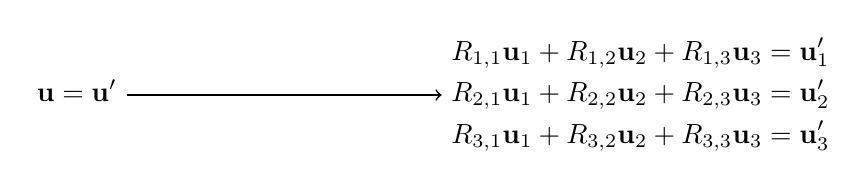
\begin{tikzpicture}[node distance=4cm]
    \node (lhs) { \(
        \begin{aligned}
            \R \point{\bvec{u}} = \point{\bvec{u}'}
        \end{aligned}
    \) };
    \node[right=of lhs] (rhs) { \(
        \begin{aligned}
             R_{1,1} \bvec{u}_1 + R_{1,2} \bvec{u}_2 + R_{1,3} \bvec{u}_3 &= \bvec{u}'_1 \\
             R_{2,1} \bvec{u}_1 + R_{2,2} \bvec{u}_2 + R_{2,3} \bvec{u}_3 &= \bvec{u}'_2 \\
             R_{3,1} \bvec{u}_1 + R_{3,2} \bvec{u}_2 + R_{3,3} \bvec{u}_3 &= \bvec{u}'_3
        \end{aligned}
    \) };
    \draw[->, semithick] (lhs.east) -- (rhs.west);
\end{tikzpicture}

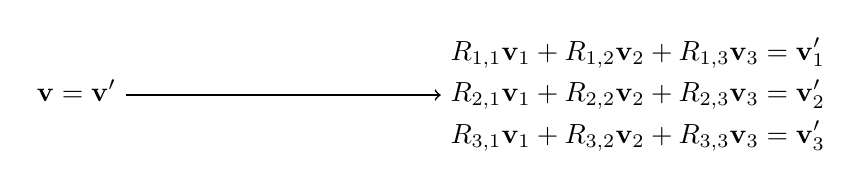
\begin{tikzpicture}[node distance=4cm]
    \node (lhs) { \(
        \begin{aligned}
            \R \point{\bvec{v}} = \point{\bvec{v}'}
        \end{aligned}
    \) };
    \node[right=of lhs] (rhs) { \(
        \begin{aligned}
             R_{1,1} \bvec{v}_1 + R_{1,2} \bvec{v}_2 + R_{1,3} \bvec{v}_3 &= \bvec{v}'_1 \\
             R_{2,1} \bvec{v}_1 + R_{2,2} \bvec{v}_2 + R_{2,3} \bvec{v}_3 &= \bvec{v}'_2 \\
             R_{3,1} \bvec{v}_1 + R_{3,2} \bvec{v}_2 + R_{3,3} \bvec{v}_3 &= \bvec{v}'_3
        \end{aligned}
    \) };
    \draw[->, semithick] (lhs.east) -- (rhs.west);
\end{tikzpicture}

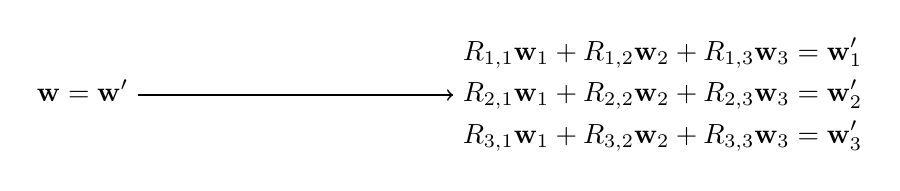
\begin{tikzpicture}[node distance=4cm]
    \node (lhs) { \(
        \begin{aligned}
            \R \point{\bvec{w}} = \point{\bvec{w}'}
        \end{aligned}
    \) };
    \node[right=of lhs] (rhs) { \(
        \begin{aligned}
             R_{1,1} \bvec{w}_1 + R_{1,2} \bvec{w}_2 + R_{1,3} \bvec{w}_3 &= \bvec{w}'_1 \\
             R_{2,1} \bvec{w}_1 + R_{2,2} \bvec{w}_2 + R_{2,3} \bvec{w}_3 &= \bvec{w}'_2 \\
             R_{3,1} \bvec{w}_1 + R_{3,2} \bvec{w}_2 + R_{3,3} \bvec{w}_3 &= \bvec{w}'_3
        \end{aligned}
    \) };
    \draw[->, semithick] (lhs.east) -- (rhs.west);
\end{tikzpicture}
\endgroup

Notice now that we have three relations for each three rows of coefficients in \( R \). This let's us now rearrange the nine equations we have as the following three systems of three equations, which we can again put back into matrix form.
\begingroup
\newcommand{\point}[1]{\ensuremath{\begin{bmatrix} #1_1 \\ #1_2 \\ #1_3 \end{bmatrix}}}
\newcommand{\pointsub}[2]{\ensuremath{\begin{bmatrix} #1_{#2,1} \\ #1_{#2,2} \\ #1_{#2,3}  \end{bmatrix}}}
\newcommand{\A}{\ensuremath{\begin{bmatrix} \bvec{u}_1 & \bvec{u}_2 & \bvec{u}_3 \\ \bvec{v}_1 & \bvec{v}_2 & \bvec{v}_3 \\ \bvec{w}_1 & \bvec{w}_2 & \bvec{w}_3 \end{bmatrix}}}

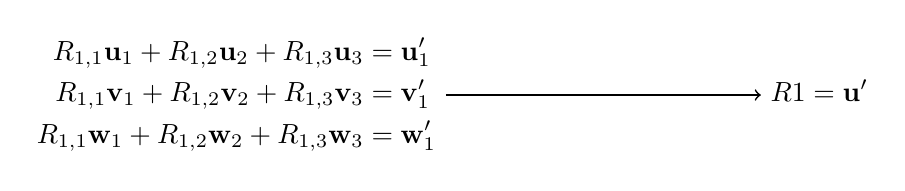
\begin{tikzpicture}[node distance=4cm]
    \node (lhs) { \(
        \begin{aligned}
            R_{1,1} \bvec{u}_1 + R_{1,2} \bvec{u}_2 + R_{1,3} \bvec{u}_3 &= \bvec{u}'_1 \\
            R_{1,1} \bvec{v}_1 + R_{1,2} \bvec{v}_2 + R_{1,3} \bvec{v}_3 &= \bvec{v}'_1 \\
            R_{1,1} \bvec{w}_1 + R_{1,2} \bvec{w}_2 + R_{1,3} \bvec{w}_3 &= \bvec{w}'_1
        \end{aligned}
    \) };
    \node[right=of lhs] (rhs) { \(
        \begin{aligned}
            \A \pointsub{R}{1} = \point{\bvec{u}'}
        \end{aligned}
    \) };
    \draw[->, semithick] (lhs.east) -- (rhs.west);
\end{tikzpicture}

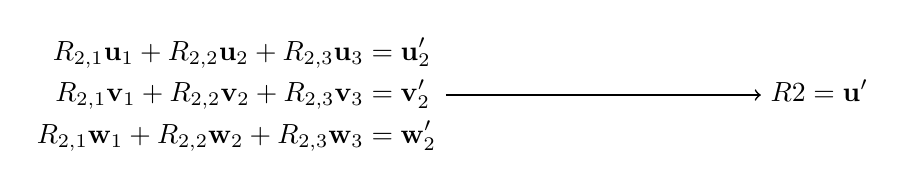
\begin{tikzpicture}[node distance=4cm]
    \node (lhs) { \(
        \begin{aligned}
            R_{2,1} \bvec{u}_1 + R_{2,2} \bvec{u}_2 + R_{2,3} \bvec{u}_3 &= \bvec{u}'_2 \\
            R_{2,1} \bvec{v}_1 + R_{2,2} \bvec{v}_2 + R_{2,3} \bvec{v}_3 &= \bvec{v}'_2 \\
            R_{2,1} \bvec{w}_1 + R_{2,2} \bvec{w}_2 + R_{2,3} \bvec{w}_3 &= \bvec{w}'_2
        \end{aligned}
    \) };
    \node[right=of lhs] (rhs) { \(
        \begin{aligned}
            \A \pointsub{R}{2} = \point{\bvec{u}'}
        \end{aligned}
    \) };
    \draw[->, semithick] (lhs.east) -- (rhs.west);
\end{tikzpicture}

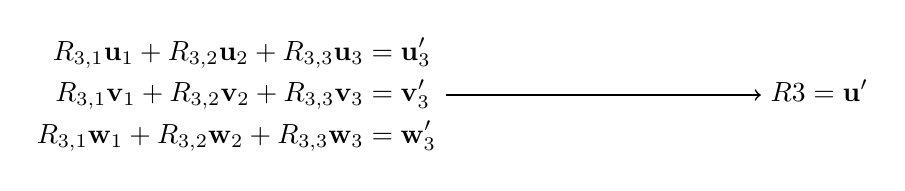
\begin{tikzpicture}[node distance=4cm]
    \node (lhs) { \(
        \begin{aligned}
            R_{3,1} \bvec{u}_1 + R_{3,2} \bvec{u}_2 + R_{3,3} \bvec{u}_3 &= \bvec{u}'_3 \\
            R_{3,1} \bvec{v}_1 + R_{3,2} \bvec{v}_2 + R_{3,3} \bvec{v}_3 &= \bvec{v}'_3 \\
            R_{3,1} \bvec{w}_1 + R_{3,2} \bvec{w}_2 + R_{3,3} \bvec{w}_3 &= \bvec{w}'_3
        \end{aligned}
    \) };
    \node[right=of lhs] (rhs) { \(
        \begin{aligned}
            \A \pointsub{R}{3} = \point{\bvec{u}'}
        \end{aligned}
    \) };
    \draw[->, semithick] (lhs.east) -- (rhs.west);
\end{tikzpicture}

Notice now that we have the same matrix on the right side. We'll call this
matrix \( A \). The great thing about this operation is that we only really
need to find the inverse of one matrix, namely \( A^{-1} \). Doing so, we
finally get a way to calculate the coefficients in \( R \) in terms of our vectors \( \bvec{u} \), \( \bvec{v} \), and \( \bvec{w} \) as such:
\[
    \pointsub{R}{1} = A^{-1} \point{\bvec{u}'}, \qquad \pointsub{R}{2} = A^{-1} \point{\bvec{v}'}, \qquad \pointsub{R}{3} = A^{-1} \point{\bvec{w}'} 
\]
\endgroup

With this, our Rubik's cube rotations now work properly \MarginComment{Okay for
the project it also actually took me a while to realize that I defined matrix
multiplication incorrectly, but we won't go into that.} and the world is saved,
with cubers and non-cubers alike able to enjoy the wonders that are rotations.


\NewSection{Generalizing Partial Fractions}{2023-05-06}

When you hear the term "partial fractions" perhaps your face lights up in
delight, or perhaps your soul fills with dread in anticipation of the drudging
through factoring and solving some linear equations for coefficients. \MarginComment{Personally, I quite enjoy doing partial fractions by hand, but to each their own I guess.} Whatever the case, partial fractions are quite the useful tool, especially so for integration and generating functions among others. However, it isn't all the time that we are working with some explicit values for our rational functions. This leads us mathematicians to a natural question, is there a way to generalize the solving of such partial fractions?

\subsection{Finding a Beautiful Result}

Let's start with the following: suppose that our rational function that we want
to decompose is of the form \( P \left( z \right) / Q \left( z \right) \),
where \( P \left( z \right) \) and \( Q \left( z \right) \) are polynomials.
Because we want to be able to factor the denominator, let us also suppose that \( Q \left( z \right) \) is a degree \( n \) polynomial with distinct, complex roots \( z_1, z_2, \ldots, z_n \). \MarginComment{Notice that I said distinct roots. While what we're doing could probably be extended, this method as of right now probably does not work for roots of greater multiplicity than one. Perhaps a problem for future me.} In short, \( Q \left( z \right) = \left( z - z_1 \right) \left( z - z_2 \right) \cdots \left( z - z_n \right) \). Then by our usual partial fractions setup, we must have that
\[
    \frac{P \left( z \right)}{Q \left( z \right)} = \sum_{i = 1}^{n} \frac{a_i}{z - z_i}
,\]
where each \( a_i \) is really just some coefficient that we don't know yet.
Most of our work will be to use some method to find these coefficients. If we
remember back to regular partial fractions, one of the first things we do after
setting it up is multiplying across by the denominator. This then later on
allows us to plug in values for \( z \) without getting \( 0 \) in the
denominator. Doing so, we get the following:
\[
    P \left( z \right) = \sum_{i = 1}^{n} a_i \cdot \frac{Q \left( z \right)}{z -  z_i}
.\]
Now we can "plug in" our \( z \) values to help us find the value for each \( a_i \). Notice the quotes around "plug in." Given that we're plugging in roots for \( z \), we really have to be careful about simply just letting \( z \) equal some value with the roots in the denominator. Instead, for each \( a_i, i \in \{ 1, 2, \ldots, n \} \), we \textit{take the limit} as \( z \) approaches the \( i \)th root \( z_i \).
\[
    \lim_{z \to z_i} P \left( z \right) = \lim_{z \to z_i} \sum_{j = 1}^{n} a_j \cdot \frac{Q \left( z \right)}{z - z_j}
.\]
Now we have something quite interesting in particular. Notice that, because \( z_i \) is a root of \( Q \left( z \right) \), each numerator goes to \( 0 \), but before we get too ahead of ourselves, we must also consider the denominator. Only when \( j = i \) does \( z_j = z_i \) and make the denominator \( 0 \). This gives us the opportunity to cancel out all but the \( j = i \) case and then consider the limit from there.
\[
    P \left( z_i \right) = a_i \cdot \lim_{z \to z_i} \frac{Q \left( z \right)}{z - z_i}
\]
This is a classic \( 0 / 0 \) indeterminate form, so we can perhaps cheekily
apply L'Hôpital's rule, which doesn't require much work at all. Solving for
each \( a_i \) then yields
\[
    a_i = \frac{P \left( z_i \right)}{Q' \left( z_i \right)}
.\]
As such, we've delivered on the goal we set out to fulfill; that is, we have found our closed form for the coefficients, which is really all we needed for partial fractions. Thus we have this general formula for partial fractions:
\[
    \frac{P \left( z \right)}{Q \left( z \right)} = \sum_{i = 1}^{n} \frac{P \left( z_i \right)}{Q' \left( z_i \right) \left( z - z_i \right)}
.\]
At least for me, the first time I saw this and figured it out on paper was
quite exciting but also I felt this was rather beautiful. The simple decomposition of a rational function somehow involves a derivative showing up in the denominator was extremely surprising to me at the time, and I've ended up using this in quite a few places.

If you know some complex analysis, you'll probably be able to see that this is related to the residues of the function. That's why this method of partial fraction decomposition is called the \textit{residue method}.

\subsection{Applications}

Now it very well wouldn't be fair to the reader, myself, or even the math
itself to show this result and not do anything with it, given how useful it
certainly can be. In the introduction I mentioned that these are particularly
useful for integration among others, so we'll go with that here. Now, if we're
talking about integration over rational functions, then there's a
\textit{really} good example of where this has benefits over your usual partial
fraction methods.
\begin{blackbox}
\begin{problem}
    Let's evaluate the infamous bump function integral using our new partial fraction method!
    \[
        \int \frac{1}{x^4 + 1} \, dx
    \]
\end{problem}
\end{blackbox}
It should be clear that we have \( P \left( x \right) = 1 \), \( Q \left( x
\right) = x^4 + 1 \), and \( Q' \left( x \right) = 4x^3 \). The first thing we'll want to do is factor our
denominator, which isn't too much different from the roots of unity.
\begin{align*}
    x^4 &= -1 =  \exp{\bigl( i \left( \pi + 2 \pi k \right) \bigr)} \\
    x  &= \exp{\bigl( i \left( \pi / 4 + k \pi / 2  \right) \bigr)}
\end{align*}
Choosing different \( k \) values from \( 0 \) to \( 3 \) gives us the \( 4 \)
distinct roots of \( Q \left( x \right) \). We will denote these roots by \(
x_0, x_1, x_2, \) and \( x_3 \), with the subscript corresponding to the value
of \( k \). Just like the roots of unity, these roots have some nice properties that interplay with each other. In particular, we have:
\begin{multicols}{2}
    \textit{Conjugates:}
    \begin{align*}
        x_0 &= \conj{x_3} \\
        x_1 &= \conj{x_2}
    \end{align*}

    \textit{Opposites:}
    \begin{align*}
        x_0 &= -x_2 \\
        x_1 &= -x_3
    \end{align*}

    \textit{Inverses:}
    \begin{align*}
        x_0 &= 1 / x_3 \\
        x_1 &= 1 / x_2
    \end{align*}

    \textit{Rotations:}
    \begin{alignat*}{2}
        x_0^3 &= x_1 &&\quad x_2^3 = x_3 \\
        x_1^3 &= x_0 &&\quad x_3^3 = x_2
    \end{alignat*}
\end{multicols}
With this in mind, we can proceed with the integral, using our residue method for partial fractions.
\begin{align*}
    \int \frac{1}{x^4 + 1} \, dx &= \int \left( \frac{1}{4x_0^3 \left( x - x_0 \right)} + \frac{1}{4x_1^3 \left( x - x_1 \right)} + \frac{1}{4x_2^3 \left( x - x_2 \right)} + \frac{1}{4x_3^3 \left( x - x_3 \right)} \right) \, dx \\
    &= \frac{1}{4} \int \left( \frac{x_3^3}{x - x_0} + \frac{x_2^3}{x - x_1} + \frac{x_1^3}{x - x_2} + \frac{x_0^3}{x - x_3} \right) \, dx \\
    &= \frac{1}{4} \int \left( \frac{x_2}{x - x_0} + \frac{x_3}{x - x_1} + \frac{x_0}{x - x_2} + \frac{x_1}{x - x_3} \right) \, dx \\
    &= \frac{1}{4} \int \left( \frac{-x_0}{x - x_0} + \frac{-x_1}{x - x_1} + \frac{x_0}{x - x_2} + \frac{x_1}{x - x_3} \right) \, dx \\
    &= \frac{x_0}{4} \Bigl( \Log{\left( x - x_2 \right)} - \Log{\left( x - x_0 \right)} \Bigr) + \frac{x_1}{4} \Bigl( \Log{\left( x - x_3 \right)} - \Log{\left( x - x_1 \right)} \Bigr) + C
\end{align*}
Now, there's a few things to pay attention to here, especially if you've seen
the antiderivative of this bump function in a different form.
\MarginComment{The "real" form that you may familiar with that includes the \(
    \ln \) and \( \arctan \) terms can be obtained by combining some of the
rational functions in the third line, but we want to avoid doing that because
it takes a whole lot more work. Besides, both of these terms are really
encompassed in the complex log anyways.} Because we've chosen to split the
function into rational functions with complex coefficients as opposed to
rational quadratics with real coefficients, we have to deal with some of the
complications of working in the complex world. Notice how our logarithm is
capitalized and doesn't have the absolute value sign. Yes, that's right, this
is not your household "real" natural logarithm but rather the complex
logarithm, defined as follows.
\[ \Log{\left( z \right)} \coloneqq \ln{\abs{z}} + i\Arg{z} .\]
More specifically, this is the principal branch where choose \( \Arg{z} \in
\left( - \pi, \pi \right] \). We're still integrating along the real line and
there isn't any contour action going on, but when dealing with the complex
logarithm and complex numbers in real integrals, we do sometimes have to be
careful about how we handle things. \MarginComment{Make sure to NINT before
doing anything major. It saves lives, folks.} Indeed, a good indicator that
something has terribly wrong and blown up is if we get a non-real value for a
real definite integral.

While we could just as easily stop here (in fact this would be great for a
computer to use), many might---rightfully so in my opinion---complain that this
is simply an unsatisfactory form that hides away what's really going on in a
more complex (heh) way. After all, if we started with a completely real
integrand, why should it be that we have an antiderivative that has complex
numbers and multi-valued functions interspersed around in it? So, with this, we shall use the power of algebra to work this into a more real-looking form.

If we are to clear this up without going through pages of algebra, it is best
that we work at the more general level and then going through specific
simplifications. Because of this, let us consider one of the general \(
\Log{\left( x - x_k \right)} \) terms. In order to not confuse what is really
going on, we shall also decompose the complex number \( x_k \) into its real and imaginary parts \( c_k + i s_k \).
\begin{align*}
    \Log{\left( x - x_k \right)} &= \ln{\abs{x - x_k}} + i \Arg{\left( x - x_k \right)} \\
    &= \ln{\abs{x - c_k + i s_k}} + i \Arg{\left( x - c_k + i s_k \right)} \\
    &= \ln{\abs{\sqrt{\left( x - c_k \right)^2 + s_k^2}}} + i \Arg{\left( x - c_k - i s_k \right)}
.\end{align*}
Inside the natural logarithm a bit of simplifying then happens, expanding the
square inside and using the fact that \( c_k^2 + s_k^2 = 1 \). Note that we
must also keep the absolute value sign when we pull out the square root and
make it a \( 1/2 \).
\begin{align*}
    \Log{\left( x - x_k \right)} &= \frac{1}{2} \ln{\abs{x^2 - 2 c_k x + 1}} + i \Arg{\left( x - c_k - i s_k \right)}
.\end{align*}
Here's where we run into just a little bit of trouble. Ordinarily, we could
turn this \( \Arg z \) term into a more comfortable single-valued real
"feeling" function like \( \arctan{\bigl( \Im \left( z \right) / \Re \left( z
\right) \bigr)} \), but we run into trouble when for example \( \Re \left( z
\right) < 0 \) and \( \Im \left( z \right) < 0 \), mapping to a positive
argument despite having a negative angle. After all, the range of \( \Arg z \)
is larger than regular old \( \arctan \). Not to mention that there is a
discontinuity if we try to do this, having a \( x - c_k \) term in the
denominator.

We can somewhat address this by using a certain \( \arctan \) identity,
\MarginComment{I'm not too sure on the rigour of this also considering that
this doesn't really solve the range problem, but the real antiderivative
matches so perhaps it's just me being confused somewhere. Perhaps something to
look at later.} which allows us to flip around its argument. Recall that
\[
    \arctan{x} = -\bigl( \pi/2 + \arctan{\left( 1/x \right)} \bigr)
\]
Using this we can now simplify the right term, giving us something that does
look suspiciously familiar to the "real" antiderivative.
\begin{align*}
    \Log{\left( x - x_k \right)} &= \frac{1}{2} \ln{\abs{x^2 - 2c_k x + 1}} - i \pi / 2 - i\arctan{\left( \frac{x - c_k}{-s_k} \right)} \\
    &= \frac{1}{2} \ln{\abs{x^2 - 2c_k x + 1}} - i \pi / 2 + i \arctan{\left( \frac{x - c_k}{s_k} \right)}
.\end{align*}
Since we have worked quite generally now, all that is left is to expand
everything out and simplify, which is a matter of just a bit of algebra. In the
end, the cancelling and the simplifying does work out to be quite satisfying,
and I won't omit it just in case the reader wants to follow along. Perhaps this
will just turn into a page of just equations, though. Who knows!
\MarginComment{Both me after writing this and the reader know.}
\begin{align*}
    &= \frac{x_0}{4} \Bigl( \Log{\left( x - x_2 \right)} - \Log{\left( x - x_0 \right)} \Bigr) + \frac{x_1}{4} \Bigl( \Log{\left( x - x_3 \right)} - \Log{\left( x - x_1 \right)} \Bigr) + C \\
    &= \frac{x_0}{4} \left( \frac{1}{2} \ln{\abs{x^2 - 2c_2 x + 1}} - i \pi/2 + i\arctan{\left( \frac{x - c_2}{s_2} \right)} \right) \\
    &- \frac{x_0}{4} \left( \frac{1}{2} \ln{\abs{x^2 - 2c_0 x + 1}} - i \pi/2 + i\arctan{\left( \frac{x - c_0}{s_0} \right)} \right) \\
    &+ \frac{x_1}{4} \left( \frac{1}{2} \ln{\abs{x^2 - 2c_3 x + 1}} - i \pi/2 + i\arctan{\left( \frac{x - c_3}{s_3} \right)} \right) \\
    &- \frac{x_1}{4} \left( \frac{1}{2} \ln{\abs{x^2 - 2c_1 x + 1}} - i \pi/2 + i\arctan{\left( \frac{x - c_1}{s_1} \right)} \right) + C \\
    &= \frac{1}{4 \sqrt{2}} \left( \frac{1}{2} \ln{\abs{x^2 + \sqrt{2} x + 1}} - i\arctan{\left( \sqrt{2} x + 1 \right)} \right) + \frac{i}{4 \sqrt{2}} \left( \frac{1}{2} \ln{\abs{x^2 + \sqrt{2} x + 1}} - i\arctan{\left( \sqrt{2} x + 1 \right)} \right) \\
    &- \frac{1}{4 \sqrt{2}} \left( \frac{1}{2} \ln{\abs{x^2 - \sqrt{2} x + 1}} + i\arctan{\left( \sqrt{2} x - 1 \right)} \right) - \frac{i}{4 \sqrt{2}} \left( \frac{1}{2} \ln{\abs{x^2 - \sqrt{2} x + 1}} + i\arctan{\left( \sqrt{2} x - 1 \right)} \right) \\
    &- \frac{1}{4 \sqrt{2}} \left( \frac{1}{2} \ln{\abs{x^2 - \sqrt{2} x + 1}} - i\arctan{\left( \sqrt{2} x - 1 \right)} \right) + \frac{i}{4 \sqrt{2}} \left( \frac{1}{2} \ln{\abs{x^2 - \sqrt{2} x + 1}} - i\arctan{\left( \sqrt{2} x - 1 \right)} \right) \\
    &+ \frac{1}{4 \sqrt{2}} \left( \frac{1}{2} \ln{\abs{x^2 + \sqrt{2} x + 1}} + i\arctan{\left( \sqrt{2} x + 1 \right)} \right) - \frac{i}{4 \sqrt{2}} \left( \frac{1}{2} \ln{\abs{x^2 + \sqrt{2} x + 1}} + i\arctan{\left( \sqrt{2} x + 1 \right)} \right) + C \\
    &= \boxed{\frac{1}{4 \sqrt{2}} \ln{\abs{x^2 + \sqrt{2} x + 1}} - \frac{1}{4 \sqrt{2}} \ln{\abs{x^2 - \sqrt{2} x + 1}} + \frac{1}{2 \sqrt{2}} \arctan{\left( \sqrt{2} x + 1\right) } + \frac{1}{2 \sqrt{2}} \arctan{\left( \sqrt{2} x - 1 \right)} + C.}
\end{align*}
Thus, we finally have our desired simplified form. 

Really this started out more as a showcase of the cool partial fractions
generalization, but it seems that in the end it morphed into simplifying our
antiderivative into its rather beautiful real result. In the end, though, I
hope your main takeaway from is that the complex logarithm form is a
beautifully compact and rather simple way of denoting this far more involved
antiderivative, and it was all thanks to the beautiful result we developed in
the first section.


\NewSection{Polynomial Differential Equations}{2023-03-29}

I'd like to think that this is a decently interesting question that stems from
some other stuff I've worked with in differential equations, we sometimes have
ODEs of the form
\[
    a_0y + a_1y' + \cdots + a_n y^{\left( n \right)} = 0
.\]
These are readily solveable using a method called the \textit{characteristic
polynomial}, \MarginComment{As we'll see later, there will be a few analogues
to these differential equations and characteristic polynomials in this
solution. Connections in math are fun!} which I won't get into too much here
(but perhaps another time?), where essentially we just assume an exponential
solution utilizing the roots of a similar looking polynomial.

Here's where sort of my inspiration comes in. Instead of looking at
differential equations that have characteristic polynomials or potential
polynomials in \( x \), what if we look at differential equations that are
\textit{polynomials in \( y \)}?

\subsection{Polynomials in \( y \)}

\begin{blackbox}
    \begin{problem}
        What can we say about differential equations of the following form and
        their solutions?
        \[
            \frac{dy}{dx} = a_0 + a_1 y + \cdots + a_n y^n
        .\]
    \end{problem}
\end{blackbox}

Because the right side is written completely in terms of \( y \), we can
recognize that this is simply a first order separable differential equation.
With this, we can move the polynomial to the left hand side by dividing and
then simply just integrate with respect to y. Then our problem lies in finding
out how to integrate this general rational function. Now where have we heard
that?

Using the same result, \MarginComment{I was quite excited when I derived it
myself, so I've used it quite a bit in various places. It's quite fun.} from
the previous journal entry, we can integrate this rational function assuming we
know the roots of the polynomial in \( y \), which we will denote as \( y_1,
y_2, \ldots, y_n \). Thus we have that
\[
    \frac{1}{a_n \left( y - y_1 \right) \left( y - y_2 \right) \cdots \left( y - y_n \right)} \cdot \frac{dy}{dx} = 1
.\]


\NewSection{A Pretty Fun Game, IMO}{2023-06-09}

\newcommand{\boxdiagram}[7][]{
    \begin{center}
    \begin{tikzpicture}
        \draw[thick] (0, 0) rectangle (1, 1);
        \draw[thick] (2, 0) rectangle (3, 1);
        \draw[thick] (4, 0) rectangle (5, 1);
        \draw[thick] (6, 0) rectangle (7, 1);
        \draw[thick] (8, 0) rectangle (9, 1);
        \draw[thick] (10, 0) rectangle (11, 1);

        \node at (0.5, 0.5) {#2};
        \node at (2.5, 0.5) {#3};
        \node at (4.5, 0.5) {#4};
        \node at (6.5, 0.5) {#5};
        \node at (8.5, 0.5) {#6};
        \node at (10.5, 0.5) {#7};

        \ifthenelse{\equal{#1}{}}{}{
            \draw[thick, ->] (5.5, -0.25) -- (5.5, -1.25);
            \node at (6, -0.75) {\ensuremath{#1}};
        }
    \end{tikzpicture}
    \end{center}
}

Hay hay! It's the summer, so I actually have quite a bit more time now to spend
on problems and such. \MarginComment{I'm actually really excited! I've vowed to
be more productive over the summer so this seems like the perfect opportunity,
although I do have to self-study some stuff.} With this extra time, I thought
it would be really cool to try and tackle a far harder competition math problem
than usual. After looking through a couple problems, I chanced upon a very cool
looking IMO problem, so I thought it would be perfect for the occasion. Here's
how it goes:

\begin{blackbox}
    \begin{problem}[2010 IMO Problem \#5]
        Each of the six boxes \( B_1, B_2, B_3, B_4, B_5, B_6 \) initially
        contains one coin. The following operations are allowed:

        \begin{enumerate}[topsep=10pt, itemsep=5pt]
            \item Choose a non-empty box \( B_j \), \( 1 \leqslant j \leqslant 5 \), remove
                one coin from \( B_j \) and add two coins to \( B_{j + 1} \).
            \item Choose a non-empty box \( B_k \), \( 1 \leqslant k \leqslant 4 \), remove
                one coin from \( B_k \) and swap the contents (maybe empty) of
                the boxes \( B_{k+1} \) and \( B_{k+2} \).
        \end{enumerate}

        Determine if there exists a finite sequence of operations of the
        allowed types, such that the five boxes \( B_1, B_2, B_3, B_4, B_5 \)
        become empty, while box \( B_6 \) contains exactly \(
        2010^{2010^{2010}} \) coins.
    \end{problem}
\end{blackbox}

As a brief remark on notation, I'll represent first move type by \( D_k \) and the second by \( S_k \), representing "double" and "swap" respectively, with \( k \) denoting the chosen box that the move acts upon.

I chose this problem in particular because, as you might see, there isn't any
crazy algebra or geometry or number theory going on where I would have to
recall some very specific theorem and have a great deal of intuition for the
subject (not to harp on those problems \textit{too much}; I just wouldn't be
able to solve them very well haha). This problem is quite nice in that it
requires, at least on its face, no mathematical background or knowledge but
rather a determined enough problem solver. It's a fun puzzle, and I really would
like to tackle it. So, let's get started!

\subsection{Observations}

It's time to brainstorm how to actually start the problem and sort of what I
think we're really aiming for. \MarginComment{To be honest, starting the problem
is probably one of my weak spots, although that may be the case somewhat for
everyone.} This problem is really a game with a set of rather simple moves, and
I get the feeling that this is going to be solved through pure logic rather
than any fancy or flashy math theorem. 

Because this is an IMO problem, I'm of the opinion that the answer is one of
two things:
\begin{enumerate}
    \item There \textit{does} exist such a sequence and it's rather hard to
        find.
    \item There \textit{doesn't} exist such a sequence, and the proof for such
        is rather hard.
\end{enumerate}
So, in summary, the problem is hard, but I mean that's why I picked it. I'm
leaning towards there being such a sequence because that seems a lot more fun,
but we probably wouldn't have to construct such a sequence anyways.

The proof may also revolve around some very light number theory in terms of
parity. We might also have to take into consideration ideas such as the maximum
possible number of coins to exist in the system and comparing that to our big
constant.

In fact, on the topic of The Big Constant\texttrademark, I find it somewhat
hard to imagine it being special or completely unique in some way that allows
this problem to work. \MarginComment{I mean if it is though that's pretty
amazing.} It's likely that, if the sequence does indeed exist, we're looking
for a more general way to reach a state of say \( 1, 1, 1, 1, 1, n \) or
something similar rather than the exact number.

Another thing to consider is that the first box may be some place to start as
there is only one possible move you can ever do on in throughout the course of
the game. When we do this move, the box ends up with \( 0 \) coins, and there
is no way to add back to that (and obviously we have to do a move on this box
because it has to become empty at some point.).

Another thing to consider is the associativity and the commutativity of the
moves. While I'm sure this problem could be framed entirely in a group theory or
abstract algebra setting, there isn't all too much to gain from doing so, but
taking some ideas over certainly can't hurt.

\subsection{Odds and Ends}

Let's start with the following observation: \( 2010^{2010^{2010}} \) is even,
and \( 1 \) is not. It sounds quite obvious, but notice that the only way we
can add pieces is with the doubling move, which adds \( 2 \) coins to the next
box. This means that the parity of the boxes stays the same in this case, which
we certainly don't want. We can address this then \MarginComment{The good 'ol
Canadian shuffle, as they call it.} by subtracting one, which does change the
parity, and then swapping the boxes around to get it into the desired position
as such:

\vspace{0.3cm}

\boxdiagram[D_5]{1}{1}{1}{1}{1}{1}
\boxdiagram[S_4]{1}{1}{1}{1}{0}{3}
\boxdiagram     {1}{1}{1}{0}{3}{0}

\let\boxdiagram\undefined


\NewSection{A Putnam Functional Integral}{2023-06-12}

Every so often, I'm scrolling through YouTube, and I find a cool problem in the
thumbnail that I just can't help but want to solve. Surprising as it is, some
Putnam problems are actually not as difficult as you might think, and the
calculus problems especially are always quite a bit of fun. Besides, it seems
I'm on quite the roll for cool competition math problems, so I might as well
continue on.

The problem that caught my eye goes as follows:

\begin{blackbox}
    \begin{problem}[77th Putnam Problem A3]
        Let \( f \colon \mathbb{R} \to \mathbb{R} \) be the solution to the functional equation
        \[
            f \left( x \right) + f \left( 1 - \frac{1}{x}  \right) = \arctan{x}
        .\]
        Find
        \[
            \int_{ 0 }^{ 1 } f \left( x \right) \, dx
        .\]
    \end{problem}
\end{blackbox}

\subsection{Solving the Functional Equation}

While at first this does look a bit daunting, let's play around a bit with the
expressions inside the functions, solving for some values. Let \( x = 2 \), giving us
\[
    f \left( 2 \right) + f \left( 1/2 \right) = \arctan{2}
.\]
Now we have two unknowns, so let's try and see if there's another relation involving \( f \left( 1/2 \right) \). Let's set \( x = 1/2 \), giving us:
\[
    f \left( 1/2 \right) + f \left( -1 \right) = \arctan{\left( 1/2 \right)}
.\]
Let's go one level deeper, setting \( x = -1 \).
\[
    f \left( -1 \right) + f \left( 2 \right) = \arctan{\left(-1 \right)}
.\]
Quite interestingly, we see that we have three relations for three different
unknowns, which means that we can solve for each of them. What's more useful
for us though, is that this choice of \( 2 \) was arbitrary, meaning that we
can do this for any value of \( x \) (disregarding singularities).
\MarginComment{For many functional equations, simply playing around with
different substitutions or specific values often helps one gain a good insight
as to what's going on.}

This means that there is a quite simple way of solving for the function, and all we need to do is just take the approach from above but generalize it.

In particular, define \( g \left( x \right) = 1 - 1 / x \). Notice the
following very nice properties that emerge when we take iterated applications
of \( g \left( x \right) \).
\begin{align*}
    g \left( x \right) &= 1 - 1/x \\
    g \left( g \left( x \right) \right) &= 1 / \left( 1 - x \right) \\
    g \left( g \left( g \left( x \right) \right) \right) &= x
.\end{align*}
Any subsequent applications will go back to one of these three functions due
to, \( x \) being the identity function. Using this, we can now solve the
functional equation. We shall use our given equation, writing it in terms of
our new function \( g \left( x \right) \) and also the modified function
equations with the substitutions \( x \mapsto g \left( x \right) \) and \( x
\mapsto g \left( g \left( x \right) \right) \) to yield a system of three
equations with three unknowns.
\[
\begin{array}{ccccccl}
    f \left( x \right) & + & f \left( g \left( x \right) \right) & + & 0 & = & \arctan{x} \\
    0 & + &  f \left( g \left( x \right) \right) & + & f \left( g \left( g \left( x \right) \right) \right) & = & \arctan{\left( g \left( x \right) \right)} \\
    f \left( x \right) & + & 0 & + & f \left( g \left( g \left( x \right) \right) \right) & = & \arctan{\left( g \left( g \left( x \right) \right) \right)}
\end{array}
\]
Through some rather simple algebra, we can solve the system to see that
\[
    2 f \left( x \right) = \arctan{x} - \arctan{\left( g \left( x \right) \right)} + \arctan{\left( g \left( g \left( x \right) \right) \right)}
.\]
With this, we're a whole lot closer to getting our answer. Now all that's left is to integrate!

\subsection{Integrating Some Arctangents}

If we integrate on both sides of our solved functional equation, we can split
up each term into separate integrals and tackle each of them one-by-one.
\[
    2 \int_0^1 f \left( x \right) \, dx = \overset{\textbf{1.}}{\boxed{\int_{ 0 }^{ 1 } \arctan{x} \, dx}} - \overset{\textbf{2.}}{\boxed{\int_{ 0 }^{ 1 } \arctan{\left( 1 - \frac{1}{x} \right)} \, dx}} + \overset{\textbf{3.}}{\boxed{\int_{ 0 }^{ 1 } \arctan{\left( \frac{1}{1 - x} \right)} \, dx}}
.\]
We'll start off with the easiest one, which is just the integral of plain \( \arctan{x} \), which lends itself well to integration by parts:
\begin{flalign*}
    \textbf{1.} \int_{ 0 }^{ 1 } \arctan{x} \, dx &= \bounds{x \arctan{x}}{0}{1} - \int_{ 0 }^{ 1 } \frac{x}{x^2 + 1} \, \tikzmarknode{ibp1}{dx} & \\
    &= \frac{\pi}{4} - \bounds{\frac{1}{2} \ln{\abs{x^2 + 1}}}{0}{1} \tikzmarknode{usub1}{} & \\
    &= \boxed{\frac{\pi}{4} - \frac{1}{2} \ln{2}}. &
\end{flalign*}
Luckily, \( \arctan{x} \) is a simple inverse function, so there's not much
difficulty in using integration by parts to find its integral. This next
integral won't be the cleanest.
\begin{tikzpicture}[overlay, remember picture]
    \draw[<-, semithick] (ibp1) ++ (0.5, 0) -- ++ (2, 0) node[above left] {\footnotesize IBP} node[right, draw=black] {
    \(
    \footnotesize
        \arraycolsep=1pt
        \begin{array}{cclcccl}
            u & = & \arctan{x} & \  & du & = & dx /( x^2 + 1 ) \\
            dv & = & dx & \  & v & = & x \\
        \end{array}
    \)};

    \draw[<-, semithick] (usub1) ++ (0.2, 0) -- ++ (3.5, 0) node[above left] {\footnotesize substitution} node[right, draw=black] {
    \(
    \footnotesize
        \arraycolsep=1pt
        \begin{array}{ccl}
            w & = & x^2 + 1 \\
            dw & = & 2x \, dx
        \end{array}
    \)};
\end{tikzpicture}

For this integral, \MarginComment{TODO: Add in the boxes showing substitutions
and such. They take a bit of work to put in, but it makes stuff easier to
follow.} we'll again start with integration by parts, but a little more work is
required to get it into a nice form.
\begin{align*}
    \textbf{2.} \int_{ 0 }^{ 1 } \arctan{\left( 1 - \frac{1}{x} \right)} \, dx &= \bounds{x \arctan{\left( 1 - \frac{1}{x} \right)}}{0}{1} - \int_{ 0 }^{ 1 } \frac{1}{x + x\left( 1 - \frac{1}{x} \right)^2} \, dx
\end{align*}
For the left term, we can plug in \( x = 1 \) to get \( 0 \) for the top bound, but we must take the limit as \( x \to 0^+ \) for the second.
\begin{align*}
    \bounds{x \arctan{\left( 1 - \frac{1}{x} \right)}}{0}{1} &= - \lim_{x \to 0^+} x \arctan{\left( 1 - \frac{1}{x} \right)} \\
    &= - \lim_{x \to 0^+} \frac{\arctan{\left( 1 - 1/x \right)}}{1 / x} \\
    &= - \lim_{x \to 0^+} \frac{1}{1 + \left( 1 - \frac{1}{x} \right)^2} \\
    &= - \lim_{u \to -\infty} \frac{1}{1 + u^2} \\
    &= 0
.\end{align*}
We now return to our integral and work it into a nicer form:
\begin{align*}
    &- \int_{ 0 }^{ 1 } \frac{1}{x + x \left( 1 - \frac{1}{x} \right)^2} \, dx = - \int_{ 0 }^{ 1 } \frac{x}{x^2 + \left( x - 1 \right)^2} \, dx \\
    &= - \int_{ 0 }^{ 1 } \frac{x}{2x^2 - 2x + 1} \, dx = - \int_{ 0 }^{ 1 } \frac{2x}{\left( 2x - 1 \right)^2 + 1} \, dx \\
    &= - \int_{ 0 }^{ 1 } \frac{\left( 2x - 1 \right) + 1}{\left( 2x - 1 \right)^2 + 1} \, dx = -\frac{1}{2} \int_{ -\pi/4 }^{ \pi/4 } \left( \tan{\theta} + 1 \right) \, d\theta \\
    &= \boxed{\frac{-\pi}{4}}
\end{align*}
On to the next integral!

For this one, we'll first do a \( u \)-substitution of the entire integrand,
getting us to something perhaps a little bit more familiar looking.
\begin{align*}
    \textbf{3.} &\int_{ 0 }^{ 1 } \arctan{\left( \frac{1}{1 - x} \right)} \, dx \\
    &= \int_{\pi/4}^{\pi/2} u \csc^2{u} \, du
.\end{align*}
We'll now do just a little bit of tabular integration:
\[
\begin{array}{ccc}
    & D & I \\
    + & u & \csc^2{u} \\
    - & 1 & -\cot{u} \\
    + & 0 & -\ln{\abs{\sin{u}}}
\end{array}
\]
This means that the integral becomes
\begin{align*}
    &\left[ -u\cot{u} + \ln{\abs{\sin{u}}} \rule{0pt}{10pt} \right]_{\pi/4}^{\pi/2} \\
    &= \boxed{\frac{\pi}{4} + \frac{1}{2} \ln{2}}
,\end{align*}
which does indeed look suspiciously familiar to some of our other results.

With this, we're pretty much complete with the problem, with all that's left to
do being to substitute our values in. Taking great care to remember the \( 2 \)
we placed in front of the integral way back last section, we see that the final
answer to the problem is
\[
    \int_{0}^{1} f \left( x \right) \, dx = \frac{1}{2} \left( \frac{\pi}{4} - \frac{1}{2} \ln{2} + \frac{\pi}{4} + \frac{\pi}{4} + \frac{1}{2} \ln{2} \right) = \boxed{\frac{3 \pi}{8}}
.\]

Perhaps I'll do more Putnam problems in the future. They seem to be an
interesting intersection of higher level mathematics (including stuff like
calculus, abstract algebra, and combinatorics among others), but they
definitely seem to have a different sort of "flavor" from the competition
problems that I'm used to. Certainly, compared to the IMO and such, there are
definitely some easier problems, but I'm sure not all of them are as easy.
Perhaps I'll get to tackle the Putnam in person myself one day. Who knows?


\NewSection{Daily Puzzle Creation}{2023-06-27}

In my 7th grade math class,\MarginComment{Ah the good old days of my youth...}
there was a clock that had on each hour label a different mathematical
expression that evaluated to that hour. For example, \( 8 \) wasn't just plain
old \( 8 \), but something like \( \sqrt{64} \) instead. I've always thought
this was a fun little recreational thing to nerd out about, but it slipped out
of my mind for the longest time.

I've since thought I should revisit this idea (mostly motivated by a bit of a
running joke that I'm having) and have a little fun crafting puzzles daily.
Compared to the clock though, they'll probably be a bit on the longer side (I
also anticipate that some problems will be easier to solve than make). Let's
get started!

\subsection{Problems}
\begin{enumerate}
    % % I'm trying to see if \filbreak is a good idea (probably wont put it for
    % the solutions because they get longer), so if this makes things wack,
    % just remove it I guess.
    % Ok yeah filbreak can break some stuff
    % \filbreak
    \item Let \( n \) be the order of the smallest possible subgroup of \( \left( \mathbb{R}, \cdot \right) \). Day \( n \).

    % \filbreak
    \item Day \( A \), where \( A \) represents the area of any triangle
        tangent to the curve \( y = 1 / x \) in the first quadrant and having
        vertices at the origin, \( x \)-axis, and \( y \)-axis.

    % \filbreak
    \item Let \( m \) be the \( 4 \)th digit of \( \tau \). Day \( m \). \MarginComment{The \( 4 \)th digit from the left, in case you needed clarification. ;)}

    % \filbreak
    \item Day
        \[
            2 \exp{\left( \frac{8}{\pi} \int_{ 0 }^{ 1 } \frac{\ln{\left( 1 + x \right)}}{x^2 + 1} \, dx \right)}
        .\]
        
    % \filbreak
    \item Day \( \abs{S_5} / \abs{S_4} \), where \( S_k \) denotes the
        symmetric group with degree \( k \).

    % \filbreak
    \item Let \( S \left( p \right) \) denote the number of times a permutation
        \( p \) must be composed until it reaches the identity permutation.
        Day \( S \left( \left( 1 \: 3 \right) \left( 2 \: 4 \: 5 \right) \right) \).

    % \filbreak
    \item Day \( D \), where \( D \) denotes the absolute distance between the
        eigenvalues of the following \( 2 \times 2 \) matrix:
        \[
            \begin{bmatrix}
                12099471394 & -8623006 \\
                121153998 & 12034827395
            \end{bmatrix}
        .\]

    % \filbreak
    \item Let \( N \) denote the number of distinct Fibonacci numbers that are perfect squares. Day \( 2^N \).

    % \filbreak
    \item Let \( \Gamma \) denote the unit circle, and define \( 13 \) circles
        \( \omega_0,\omega_1,\ldots,\omega_{12} \) such that they are all of
        equal radius \( r \) and externally tangent to \( \Gamma \). \MarginComment{I am
        definitely not the most experienced in Euclidean geometry so this might
        be a weird way to phrase the question.} In addition, each circle \(
        \omega_k \) is externally tangent to \( \omega_{(k - 1) \bmod{13}} \) and \( \omega_{(k
        + 1) \bmod{13}} \). Day \( \floor{30r} \).

    \item Big Boy Bill has a counter at value \( 0 \) and flips a fair, random
        coin \( 15 \) times. Every time he flips the coin, if it lands on
        heads, he adds \( 2 \) to the counter, and if it lands on tails, he
        adds \( 3 \) to the counter. There are \( m \) different sequences of
        coin flips in which at the end of the flipping, the resulting value is
        divisible by \( 5 \). Day \( 2m \bmod{23} \).

    \item For a base \( b \geqslant 3 \), define the \textit{descending base number}
        \( D \left( b \right) \) to be the \( \left( b - 1 \right) \) digit
        number in base \( b \) where the \( i \)th digit is precisely \( i \).
        For example, \( D \left( 4 \right) = 321_4 = 57 \). Let \( P \) be the
        number of descending base numbers that are prime. Day \( P^2 - 6P + 16
        \).
\end{enumerate}

\subsection{Solutions}
\begin{enumerate}
    \item By the definition of a group, it must at least include the identity
        element, meaning that the order must be positive. In general, the
        smallest and perhaps most trivial subgroup of a group is one containing
        solely the identity element (for this specific case the group is \(
        \left( \set{1}, \cdot \right) \)), thus our answer is \( \boxed{1} \).

        We shall give a general proof that the subgroup containing just the
        identity element exists.
        \begin{proof}
            We are given a group \( \left( G, \cdot \right) \) with identity
            \MarginComment{Ehh this feels a bit elementary but it's fine.}
            element \( e \). We shall prove that \( \left( \set{e}, \cdot
            \right) \) is a group and subsequently a subgroup of \( G \). We
            already have fulfilled the identity element condition required in
            the definition of a group, so all that is left is to verify that
            the inverse of \( e \) is in the subgroup (which would mean that it is equal to \( e \)).

            Suppose that \( e^{-1} = e \), giving us
            \[
                e \cdot e^{-1} = e^{-1} \cdot e = e \cdot e = e
            .\]
            This fulfills the condition to be an inverse, and thus \( \left(
            \set{e}, \cdot \right) \) is a group and a subgroup of \( G \).
        \end{proof}

    \item Let \( a \) be some positive real number. We shall find the line
        passing through \( \left( a, 1 / a \right) \) and tangent to the curve
        \( y = 1 / x \) to be
        \[
            y = 1 / a - 1 / a^2 \left( x - a \right)
        .\]
        Setting \( x \) and \( y \) to be zero individually and solving, we
        find that there is an \( x \)-intercept at \( \left( 2a, 0 \right) \)
        and a \( y \)-intercept at \( \left( 0, 2/a \right) \). This forms a right triangle
        with area \( 1 / 2 \cdot 2a \cdot 2 / a = \boxed{2} \).

    \begin{figure}[h]
        \centering
        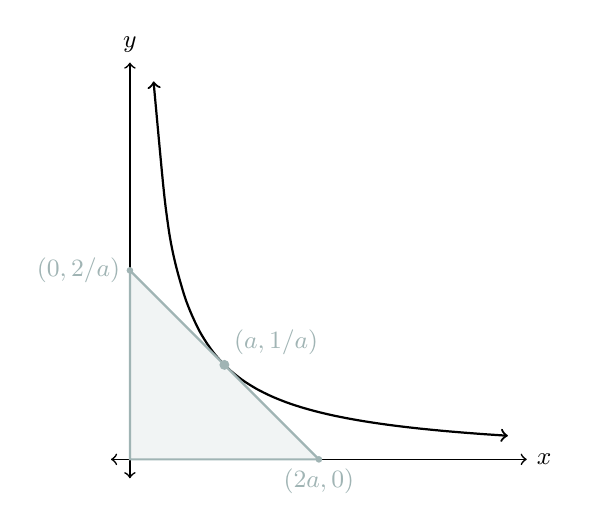
\begin{tikzpicture}[domain=0.25:4, scale=1.2]
            \draw[<->, semithick] (-0.2, 0) -- (4.2, 0) node[right] {\small \( x \)};
            \draw[<->, semithick] (0, -0.2) -- (0, 4.2) node[above] {\small \( y \)};
            \draw[<->, thick, smooth] plot (\x, 1 / \x);

            \fill[fadegray!15, thick] (2, 0) -- (0, 2) -- (0, 0) -- cycle;
            \draw[fadegray, thick] (2, 0) -- (0, 2) -- (0, 0) -- cycle;

            \fill[fadegray] (1, 1) circle (1.5pt) node[above right] {\small \( \left( a, 1/a \right) \)};
            \fill[fadegray] (2, 0) circle (1pt) node[below] {\small \( \left( 2a, 0 \right) \)};
            \fill[fadegray] (0, 2) circle (1pt) node[left] {\small \( \left( 0, 2/a \right) \)};
        \end{tikzpicture}
        \caption{An example tangent triangle for Problem 2}
    \end{figure}
    
    \item Perhaps \MarginComment{I didn't put that much effort into making this
        problem as you can probably see.} you can figure this out with proper
        analytical methods, but \( \tau \approx 6.2832 \), so uhhhh... The
        answer is \( \boxed{3} \).

    \item We parametrize the inner integral as such:
        \[
            I \left( a \right) = \int_{ 0 }^{ 1 } \frac{\ln{\left( 1 + ax \right)}}{x^2 + 1} \, dx
        ,\]
        giving us an initial condition that \( I \left( 0 \right) = 0 \). We
        can then differentiate both sides with respect to \( a \) and do some
        integrating:
        \begin{align*}
            I' \left( a \right) &= \int_{ 0 }^{ 1 } \frac{x}{( 1 + ax ) ( x^2 + 1 )} \, dx \\
            &= \frac{1}{a^2 + 1} \int_{ 0 }^{ 1 } \frac{x + a}{x^2 + 1} \, dx - \frac{a}{a^2 + 1} \int_{ 0 }^{ 1 } \frac{1}{ax + 1} \, dx \\
            &= \bounds{\frac{1}{2 ( 1 + a^2 )} \ln{\abs{x^2 + 1}}}{0}{1} + \bounds{\frac{a}{a^2 + 1} \arctan{x}}{0}{1} - \bounds{\frac{1}{a^2 + 1} \ln{\abs{1 + ax}}}{0}{1} \\
            &= \frac{\ln{2}}{2 (1 + a^2)} + \frac{\pi a}{4 (1 + a^2)} - \frac{\ln{\left( 1 + a \right)}}{a^2 + 1}
        .\end{align*}
        Now we can solve for \( I \left( 1 \right) \), which is exactly our
        desired integral. \MarginComment{Yes that is tau you see in the
        integral bounds. Tau for tau day.}
        \begin{align*}
            I \left( 1 \right) &= I \left( 0 \right) + \int_{ 0 }^{ 1 } I' \left( \tau \right) \, d\tau \\
            &= \frac{\pi \ln{2}}{8} + \frac{\pi \ln{2}}{8} - \int_{ 0 }^{ 1 } \frac{\ln{\left( \tau + 1 \right)}}{\tau^2 + 1} \, d\tau \\
            &= 2 \cdot \frac{\pi \ln{2}}{8} - I \left( 1 \right) \\
            \implies I \left( 1 \right) &= \frac{\pi \ln{2}}{8}
        .\end{align*}
        Now we can plug this in and simplify the given expression:
        \begin{align*}
            &2 \exp{\left( \frac{8}{\pi} \int_{ 0 }^{ 1 } \frac{\ln{\left( 1 + x \right)}}{x^2 + 1} \, dx \right)} \\
            &= 2 \exp{\left( \frac{8}{\pi} \cdot \frac{\pi \ln{2}}{8} \right)} \\
            &= 2 \exp{\left( \ln{2} \right)} \\
            &= \boxed{4}
        .\end{align*}

    \item The order of the symmetric group \( S_k \) is simply \( k! \), so the answer is \( 5!/4! = \boxed{5} \).

    \item One can either manually multiply the permutation out until it reaches
        the identity permutation or realize that because it is factored into
        two disjoint cycles of length \( 2 \) and \( 3 \), it will require \(
        \gcd{\left( 2, 3 \right)} = \boxed{6} \) compositions to return to the identity
        permutation.

    \item The eigenvalues of the matrix are given by the solutions to the following polynomial:
        \[
            \left( \lambda - 12099471394 \right) \left( \lambda - 12034827395 \right) + 8623006 \cdot 121153998 = 0
        .\]
        Notice that distance between the roots is exactly the discriminant, which is
        \begin{align*}
            D &= \sqrt{\left( 12099471394 + 12034827395 \right)^2 - 4 \left( 12099471394 \cdot 12034827395 + 8623006 \cdot 121153998 \right)} \\
            &= \boxed{7}
        .\end{align*}

    \item It has been proven \MarginComment{While I would have liked to give a
        proof of this statement it turns out to involve a bit of machinery.}
        that the only three perfect square Fibonacci numbers are \( 0, 1\), and
        \( 144 \). Thus, our answer is \( 2^3 = \boxed{8} \).

    \item This one took me a bit and a half to compose. \MarginComment{Future
        Rushil here. Hahahahaha I overcomplicated this solution a lot. If you
        consider a 13-gon with radius \( 1 + r \) and then find the distance
        between the vertices with some light trig, everything pops out quite well (credit
        to Kelly for that :skull:).} Essentially what I'm trying to convey is
        that the each circle \( \omega_k \) is tangent to the previous and next
        circle and the center unit circle, forming a ring of circles.

    \begin{figure}
        \begin{minipage}{0.5\textwidth}
            \centering
            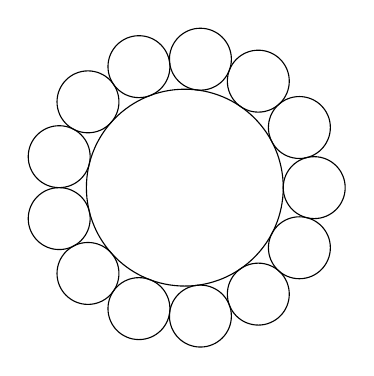
\begin{tikzpicture}[scale=1.25]
                \draw (0, 0) circle (1);

                \foreach \k in {0,...,12} {
                    \draw ({1.3146 * cos(360 * \k / 13)}, {1.3146 * sin(360 * \k / 13)}) circle (0.3146);
                }
            \end{tikzpicture}
            \caption{The idea Problem 9 is trying to convey.}
        \end{minipage}
        \begin{minipage}{0.5\textwidth}
            \centering
            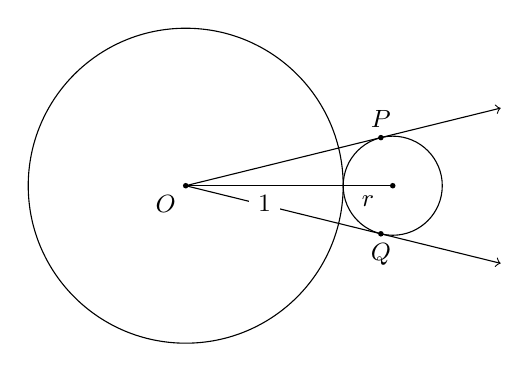
\begin{tikzpicture}[scale=2]
                \draw (0, 0) circle (1);
                \fill (0, 0) circle (0.5pt) node[below left] {\small \( O \)};

                \draw (1 + 0.3146, 0) circle (0.3146);
                \fill (1 + 0.3146, 0) circle (0.5pt);

                \draw[->] (0, 0) -- (2, {2 * 0.3146 / sqrt(2 * 0.3146 + 1)});
                \draw[->] (0, 0) -- (2, {-2 * 0.3146 / sqrt(2 * 0.3146 + 1)});
                \fill ({2 - 1 / (0.3146 + 1)}, {0.3146 / sqrt(2 * 0.3146 + 1) * (2 - 1 / (0.3146 + 1))}) circle (0.5pt) node[above] {\small \( P \)};
                \fill ({2 - 1 / (0.3146 + 1)}, {-0.3146 / sqrt(2 * 0.3146 + 1) * (2 - 1 / (0.3146 + 1))}) circle (0.5pt) node [below] {\small \( Q \)};

                \draw (0, 0) -- (1, 0) node[midway, below, fill=white] {\small \( 1 \)};
                % \node[below] at (0.5, 0) {}
                \draw (1, 0) -- (1 + 0.3146, 0) node[midway, below] {\small \( r \)};
            \end{tikzpicture}
            \caption{A diagram for the solution to Problem 9.}
        \end{minipage}
    \end{figure}

    Construct a circle, we'll call this \( \omega_0 \) of some unknown radius
    \( r \) that is externally tangent to \( \Gamma \). For simplicity, we'll
    pull it to the exact right of \( \Gamma \). Let \( O \) be the center of \(
    \Gamma \) and \( P,Q \) respectively be the points lying on the two tangent
    lines to \( \omega_0 \) extending from \( O \). Notice that \( 2 \pi /
    \angle POQ \) should be the number of circles that one can fit around \(
    \Gamma \), in other words, \( 13 \).

    Notice that if we find the slope \( a \) of \( \overrightarrow{OP} \), we
    can find \( \angle POQ = 2 \arctan{a} \). This motivates us to use analytic
    methods \MarginComment{There might be a more "geometric" solution, but this
    is the method that I used.}. 

    If we take \( O \) to be the origin, we can represent \( \omega_0 \) by
    \[
        \left( x - \left( 1 + r \right) \right)^2 + y^2 = r^2
    ,\]
    and we can let \( \overrightarrow{OP} \) be represented by the line \( y =
    ax \). If we substitute this expression for \( y \) into the equation for
    \( \omega_0 \) and set the discriminant equal to \( 0 \) (because this line
    is tangent to \( \omega_0 \)), we can obtain an expression for \( a \) in
    terms of \( r \) as follows:
    \begin{align*}
        \omega_0 \colon 0 &= \left( a^2 + 1 \right) x^2 - 2 \left( 1 + r \right)x + \left( 1 + r \right)^2 - r^2 \\
        \implies 0 &= 4 \left( 1 + r \right)^2 - 4 \left( a^2 + 1 \right) \left( 2r + 1 \right) \\
        a &= \frac{r}{\sqrt{2r + 1}}
    .\end{align*}
    We can now substitute this into our condition of \( 13 \) circles to get
    \begin{align*}
        \frac{2 \pi}{\angle POQ} &= 13 \\
        \implies \frac{\pi}{\arctan{a}} &= 13 \\
        \implies \frac{r}{\sqrt{2r + 1}} &= \tan{\left( \frac{\pi}{13} \right)}
    .\end{align*}
    Solving this for the positive root gives us \( r \approx 0.3146 \), which means that \( \floor{30r} = \boxed{9} \).

    \item Suppose BBB \MarginComment{BBB is the shorthand for Big Boy Bill, for
        those unaware.} flips \( k \) heads. Necessarily, this means he must
        have flipped \( 15 - k \) tails. From this, we can calculate the ending
        counter value and then take it modulo \( 5 \) to find the values of \(
        k \) that make our condition hold. Doing so, we can see that
        \begin{align*}
            2k + 3 \left( 15 - k \right) &\equiv 0 \pmod{5} \\
            \implies k &\equiv 0 \pmod{5}
        .\end{align*}
        As such, the only legal values of \( k \) that make the counter value
        divisible by \( 5 \) are \( 0, 5, 10 \), and \( 15 \). We're now
        looking for sequences of flips where we \textit{choose} \( 0, 5, 10 \),
        or \( 15 \) heads, which we can count to be
        \[
            \binom{15}{0} + \binom{15}{5} + \binom{15}{10} + \binom{15}{15} = 6008
        .\]
        Now all that's left is to see that \( 2 \cdot 6008 \bmod{23} = \boxed{10} \).

    \item We write the summation representation of \( D \left( b \right) \)
        first:
        \[
            D \left( b \right) = \sum_{i = 1}^{b - 1} i b^{i - 1}
        .\]
        Motivated by this representation, examine \( D \left( b \right) \)
        modulo \( \left( b - 1 \right) \). Because we are working in base \( b
        \), this is equivalent to finding the sum of the digits modulo \(
        \left( b - 1 \right) \). In other words,
        \[
            D \left( b \right) \equiv b \left( b - 1 \right) / 2 \equiv 0 \pmod{\left( b - 1 \right)}
        .\]
        In the case that \( b \) is even, this is \( 0 \), meaning that \( D
        \left( b \right) \) is not prime. We now must check the case that \( b
        \) is odd. Let \( b = 2k + 1 \). Notice that \( D \left( b \right) = D
        \left( 2k + 1 \right) \) is also the sum of its digits modulo \( k \).
        Equivalently,
        \[
            D \left( 2k + 1 \right) \equiv k \left( k - 1 \right) \equiv 0 \pmod{k}
        .\]
        Thus for odd \( b \) too, \( D \left( b \right) \) is not prime. We do,
        however, have one extraneous case for \( b = 3 = 2 \cdot 1 + 1 \).
        Since all numbers are divisible \( 1 \), we cannot apply this
        conclusion to it. Checking manually to see that \( D \left( 3 \right) =
        7 \) is prime, we have that \( P = 1 \). Thus, our answer is \( P^2 -
        6P + 16 = \boxed{11}. \)

\end{enumerate}


\NewSection{Building Geometry, Analytically}{2023-06-30}

Combinatorics is a really beautiful subject \MarginComment{I'd probably say
that in competition math, combinatorics is up there for my favorite subject} in
that, in premise, it can be very simple, but in practice it actually takes a
decent bit of thinking and cleverness sometimes. Being so widely defined as the
science of counting "things," combinatorics also lends itself very well to
intersections with other subjects. You can have geometry, number theory,
algebra, probability, and many others mixed into a combinatorics problem,
making them really fun and sometimes quite the challenge.

While it certainly is fun to solve these problems, I think it's also perhaps
quite instructive for me (and perhaps the readers) to create my own
combinatorics problems and gather a wide variety of practice problems. Creating
my own problems will be the perfect opportunity to get more acquainted with
some of the cool tricks and structure to problems, helping me in furthering my
combinatorics adventure and giving me some good exercise.
\MarginComment{Calisthenics is a category of exercises which rely primarily on
gravity and body weight. I thought it would be a funny name for this entry
mainly because my friends have roped me into it.}

In the process of making these, I'll probably put down whatever comes to mind
really, so some problems might be really easy or perhaps insanely cumbersome to
work with; nevertheless, it will still be a nice catalogue of my journey
through the world of counting.

As for solutions, I'll probably write down some of the cooler ones whenever I
have time, but I don't think I'll be able to get to all of the problems.

I hope to include not only competition math "flavored" problems which have slick
combinatorial arguments, but also some more exploratory problems perhaps using
generating functions and more of the higher level combinatorics stuff. With
that said, let's get to problem synthesizing!

\subsection{General Combinatorics}

\textit{Problems}: 
\begin{enumerate}
    \item How many partitions of the set \( \set{1, 2, \ldots, 20} \) have at
        least \( 10 \) elements?

    \item Exactly \( 12 \) of your homies, \MarginComment{For those with \( n <
        12 \), where \( n \) denotes the number of homies you have, you may
        borrow some for the sake of mathematics.} denoted \( h_1, h_2,\ldots,
        h_{12} \), are arranged in a circle. Starting from the first homie, \(
        h_1 \), and going in order, each homie pulls a string from themselves
        to another homie, so long as that string does not pass over any other
        strings in the process. All connections between homies must be made
        inside the circle. This process is continued until no more connections
        can be made. How many end states are there?
\end{enumerate}

\subsection{Geometry}

\textit{Problems}: 
\begin{enumerate}
    \item Suppose we have \( n \) circles in the plane. \MarginComment{This
        could potentially be infinite or trivial for large \( n \), but for \(
        k = 2 \), I at least know there's some interesting stuff to play around
        with.} Allowing for the adjustment of position and size of all circles, what is
        the maximum number of lines one can place that are tangent to \( k \) circles?
\end{enumerate}

\subsection{Number Theory}

\textit{Problems}: 
\begin{enumerate}
    \item How many pairs of positive integers \( \left( a, b, c \right) \) satisfy
        \[
            a + b + c = 23 \quad \text{and} \quad a + 2b + c = 40
        ?\]

    \item How many partitions of the set \( \set{1, 2, \ldots, 50} \) can one
        make where the greatest common divisor of the partition is \( 50 \)?
\end{enumerate}

\subsection{Algebra}

\textit{Problems}: 
\begin{enumerate}
    \item How many polynomials of the form
        \[
            P \left( x \right) = x^2 + ax + b
        \]
        have at least one real root, for \( a, b \in \set{1, 2, \ldots, 50} \)?
\end{enumerate}

\subsection{Colorings}

\textit{Problems}: 
\begin{enumerate}
    \item How many ways are there to color the vertices of a cube either red,
        blue, or green such that no two adjacent vertices are the same color?
\end{enumerate}

\subsection{Contest Problems}

\textit{Problems}: 
\begin{enumerate}
    \item (2019 AMC 12A \#13) How many ways are there to paint each of the
        integers \( 2,3,\ldots,9 \) either red, green, or blue so that each
        number has a different color from each of its proper divisors?
\end{enumerate}


\NewSection{Combo Calisthenics}{2023-07-06}

Combinatorics is a really beautiful subject \MarginComment{I'd probably say
that in competition math, combinatorics is up there for my favorite subject} in
that, in premise, it can be very simple, but in practice it actually takes a
decent bit of thinking and cleverness sometimes. Being so widely defined as the
science of counting "things," combinatorics also lends itself very well to
intersections with other subjects. You can have geometry, number theory,
algebra, probability, and many others mixed into a combinatorics problem,
making them really fun and sometimes quite the challenge.

While it certainly is fun to solve these problems, I think it's also perhaps
quite instructive for me (and perhaps the readers) to create my own
combinatorics problems and gather a wide variety of practice problems. Creating
my own problems will be the perfect opportunity to get more acquainted with
some of the cool tricks and structure to problems, helping me in furthering my
combinatorics adventure and giving me some good exercise.
\MarginComment{Calisthenics is a category of exercises which rely primarily on
gravity and body weight. I thought it would be a funny name for this entry
mainly because my friends have roped me into it.}

In the process of making these, I'll probably put down whatever comes to mind
really, so some problems might be really easy or perhaps insanely cumbersome to
work with; nevertheless, it will still be a nice catalogue of my journey
through the world of counting.

As for solutions, I'll probably write down some of the cooler ones whenever I
have time, but I don't think I'll be able to get to all of the problems.

I hope to include not only competition math "flavored" problems which have slick
combinatorial arguments, but also some more exploratory problems perhaps using
generating functions and more of the higher level combinatorics stuff. With
that said, let's get to problem synthesizing!

\subsection{General Combinatorics}

\textit{Problems}: 
\begin{enumerate}
    \item How many partitions of the set \( \set{1, 2, \ldots, 20} \) have at
        least \( 10 \) elements?

    \item Exactly \( 12 \) of your homies, \MarginComment{For those with \( n <
        12 \), where \( n \) denotes the number of homies you have, you may
        borrow some for the sake of mathematics.} denoted \( h_1, h_2,\ldots,
        h_{12} \), are arranged in a circle. Starting from the first homie, \(
        h_1 \), and going in order, each homie pulls a string from themselves
        to another homie, so long as that string does not pass over any other
        strings in the process. All connections between homies must be made
        inside the circle. This process is continued until no more connections
        can be made. How many end states are there?
\end{enumerate}

\subsection{Geometry}

\textit{Problems}: 
\begin{enumerate}
    \item Suppose we have \( n \) circles in the plane. \MarginComment{This
        could potentially be infinite or trivial for large \( n \), but for \(
        k = 2 \), I at least know there's some interesting stuff to play around
        with.} Allowing for the adjustment of position and size of all circles, what is
        the maximum number of lines one can place that are tangent to \( k \) circles?
\end{enumerate}

\subsection{Number Theory}

\textit{Problems}: 
\begin{enumerate}
    \item How many pairs of positive integers \( \left( a, b, c \right) \) satisfy
        \[
            a + b + c = 23 \quad \text{and} \quad a + 2b + c = 40
        ?\]

    \item How many partitions of the set \( \set{1, 2, \ldots, 50} \) can one
        make where the greatest common divisor of the partition is \( 50 \)?
\end{enumerate}

\subsection{Algebra}

\textit{Problems}: 
\begin{enumerate}
    \item How many polynomials of the form
        \[
            P \left( x \right) = x^2 + ax + b
        \]
        have at least one real root, for \( a, b \in \set{1, 2, \ldots, 50} \)?
\end{enumerate}

\subsection{Colorings}

\textit{Problems}: 
\begin{enumerate}
    \item How many ways are there to color the vertices of a cube either red,
        blue, or green such that no two adjacent vertices are the same color?
\end{enumerate}

\subsection{Contest Problems}

\textit{Problems}: 
\begin{enumerate}
    \item (2019 AMC 12A \#13) How many ways are there to paint each of the
        integers \( 2,3,\ldots,9 \) either red, green, or blue so that each
        number has a different color from each of its proper divisors?
\end{enumerate}


\NewSection{Iterating Graphs}{2023-07-18}

Recently, I've been getting into graph theory with my interest in competitive
programming and other math problems \MarginComment{Hopefully you'll see more of
this quite soon ;)}, and one day I had the idea of creating an animation of
what \textit{all} the (undirected, without loops) graphs look like for some \(
n \) vertices, and creating some aesthetically pleasing looking visualization
that moves between all of them. This journal entry was really inspired by the
math that goes behind it and how one actually goes about (somewhat) efficiently
generating these graphs.

The end result ended up turning out to be quite nice (at least in my opinion)
even if it was quite a simple visualization in idea. You can check it out here:
\url{https://chirprush.github.io/animations/animations/graph-iterations/index.html}.

\subsection{Encoding Graphs}

The idea that was sort of swimming around in my head was how one would encode a
graph as something that could be easily manipulated and played around with. One
could take the simple route, storing a bunch of vertices and then collecting
all the edges as tuples holding the vertex information, but this is quite bulky
and certainly no fun, right? Surely we can compress a graph into something
smaller than that; We just first need to revisit what exactly makes a graph a
graph.

A graph is formally defined in terms of both its vertices and its edges, which
are connections between these vertices. For our purposes of seeing "all" graphs
though, we aren't really that concerned with the infinitely many positions of
these vertices, so we can just place them evenly spaced on a circle for
convenience and the visual appeal of \( n \)-gons. With vertices out of the
way, all that really determines our different graphs is the edges that connect
our \( n \) vertices. Since we're looking for a \textit{bijection} from some
space (which we'll call \( S \)) to this space of graphs, a good motivating
question is: for \( n \) vertices, how many graphs do we exactly have?

A simple combinatorial argument helps us out here. For each pair of vertices,
you can make the binary choice to either add an edge or leave it empty. Counting the number of possible pairs gives us
\begin{align*}
    \binom{n}{2} = \frac{n \left( n - 1 \right)}{2} \> \text{ possible pairs,} && \text{giving} && 2^{n \left( n - 1 \right) / 2} \> \text{ possible graphs}
.\end{align*}
This means that, for example, there are \( 2^3 = 8 \) total possible ways to
pick the edges on a graph with \( 3 \) vertices. Note that while this does
count graphs that are isomorphic to each other, including obvious "rotations," we're fine with this. After all, our goal is to show \textit{all} graphs.

\MarginComment{
    \begin{center}
        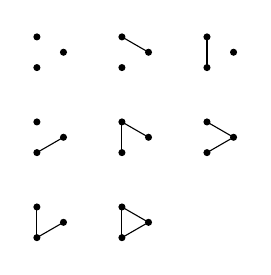
\begin{tikzpicture}[scale=0.9]
            \foreach \g in {0,...,7} {
                \foreach \i in {0,...,2} {
                    \node (\g\i) at ({1.2 * Mod(\g, 3) + 0.25 * cos(deg(\i * 2 * pi / 3))}, {-1.2 * floor(\g / 3) + 0.25 * sin(deg(\i * 2 * pi / 3))}) {};
                    \fill (\g\i) circle (0.05);
                }
            }

            \draw (10.center) -- (11.center);

            \draw (21.center) -- (22.center);

            \draw (30.center) -- (32.center);

            \draw (40.center) -- (41.center);
            \draw (41.center) -- (42.center);

            \draw (50.center) -- (51.center);
            \draw (52.center) -- (50.center);

            \draw (61.center) -- (62.center);
            \draw (62.center) -- (60.center);

            \draw (70.center) -- (71.center);
            \draw (70.center) -- (72.center);
            \draw (71.center) -- (72.center);
        \end{tikzpicture}
    \end{center}
    \captionof{figure}{All \( 8 \) possible graphs for \( 3 \) vertices.}
}

With this, we know our encoding must map from a set of \( 2^{n \left( n - 1
\right) / 2} \) elements to one unique graph, \textit{i.e.} \( \abs{S} = 2^{n
\left( n - 1 \right) / 2} \). We haven't really specified what the elements of
\( S \) should be, but one of the most useful and easy to work with choices is
simply the set of the integers \MarginComment{We will see later that this
choice to start counting from \( 0 \) is not merely because I'm a programmer.}
\[
    S = \{0, 1, \ldots, 2^{n \left( n - 1 \right) / 2} - 1 \}
.\]
This allows us to easily count up to some natural numbers and generate our
encoded graphs quite easily, which can then be decoded.

What we haven't yet chosen now is \textit{how} each number corresponds to a
graph and \textit{why}. There are quite a few ways of doing this (\( \abs{S}!
\), in fact), but we would like to choose one that makes both intuitive and
algorithmic sense. For this, we'll take a look a few steps back in our
approach, specifically to where we counted the number of graphs.

One structure associated with graphs that further illustrates the
\textit{binary} action of choosing whether or not to add an edge between two
vertices is an \textbf{adjacency matrix}. Recall that in graph theory, we
define the adjacency matrix of a simple graph to be an \( n \times n \) matrix
where each entry \( A_{ij} \) is either \( 1 \) if there exists an edge between
the \( i \)th and \( j \)th vertices and \( 0 \) if there does not. For example, for the graph \( C_4 \) (the cyclic graph with \( 4 \) vertices), the adjacency matrix is
\[
    A = \begin{bmatrix}
        0 & \tikzmark{tritop} 1 & 0 & \tikzmark{tricorn} 1 \\
        1 & 0 & 1 & 0 \\
        0 & 1 & 0 & \tikzmark{tribot} 1 \\
        1 & 0 & 1 & 0 \\
    \end{bmatrix}
.\]

\begin{tikzpicture}[remember picture, overlay]
    \fill[opacity=0.2, fadegray, rounded corners] ([xshift=-0.25cm, yshift=0.25cm]pic cs:tritop) -- ([xshift=0.2cm, yshift=0.25cm]pic cs:tricorn) -- ([xshift=0.2cm, yshift=-0.25cm]pic cs:tribot) -- cycle;
\end{tikzpicture}
Because this is a undirected graph, the matrix is symmetric about the diagonal,
and all we need to consider is one of the triangles (the one above or below the
diagonal). One can verify that this triangle has exactly the \( n \left( n - 1
\right) / 2 \) \MarginComment{A quick way to show this is that the diagonal
takes up \( n \) elements, so if we let \( T \) be the number of elements in
each triangle, we have \( 2T + n = n \times n \).} bits representing our edges.
Thus, we see something interesting here. If we \textit{flatten} the adjacency
matrix triangle, we can represent our graph as a number in binary form. This
also perfectly fits all our numbers into the domain set \( S \).

For example, in the case of the \( C_4 \) graph, we would encode it as \( G =
101101_2 = 45 \). Although in this case the number is a palindrome in base \( 2
\), we would place the bits according to the order they appear in the triangle.
The first bit (from the right) would correspond to the edge \( \set{1, 2} \),
the second corresponding to \( \set{1, 3} \), and so on.

With this, the animation also has the cool effect of sort of counting up in
binary with the edges. This also gives a somewhat natural progression from the empty graph to the complete graph for \( n \) vertices.

\MarginComment{
    \begin{center}
    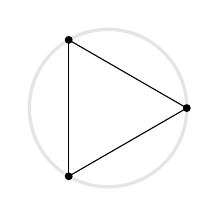
\begin{tikzpicture}
        \draw[opacity=0.1, very thick] (0, 0) circle (1);

        \node (v0) at ({1 * cos(0)}, {1 * sin(0)}) {};
        \node (v1) at ({1 * cos(deg(2 * pi / 3))}, {1 * sin(deg(2 * pi / 3))}) {};
        \node (v2) at ({1 * cos(deg(4 * pi / 3))}, {1 * sin(deg(4 * pi / 3))}) {};

        \fill (v0) circle (0.05);
        \fill (v1) circle (0.05);
        \fill (v2) circle (0.05);

        \draw (v0.center) -- (v1.center);
        \draw (v0.center) -- (v2.center);
        \draw (v1.center) -- (v2.center);
    \end{tikzpicture}
    \end{center}
    \captionof{figure}{The animation displaying the complete graph \( K_3 \), encoded as \( 111_2 = 7 \).}
}


Thus, we've found a suitable encoding for our graphs into numbers. In our
actual program, we're iterating over numbers and converting them to graphs
instead, so we'll also have to find some way of going the other way around.
Luckily, we've already built the foundation and intuition for how this will
work.

\subsection{Decoding Graph Numbers}

If the encoding stage involves taking a graph and turning it into a number
based on its adjacency matrix and edges, the decoding stage is precisely the
opposite of this: we take a number, decompose it into it's binary
representation, and turn it into an adjacency matrix, which defines the edges
and the complete representation of our graph.

There are quite a few ways do this, but in order to choose a sensible one,
we'll look at the edges of the graphs, specifically the vertices that they
connect. If we number (quite arbitrarily) the vertices of a graph \(
1,2,\ldots,n \), we have the following unique (undirected) edges:
\[
\begin{array}{cccc}
    \set{1, 2}, & \set{1, 3}, & \cdots, & \set{1, n} \\
    \set{2, 3}, & \cdots, & \set{2, n} & \\
    \vdots & \udots & \\
    \set{n - 1, n} & & &
\end{array}
\]
We want each bit of our "number to be decoded" to correlate to an edge in this
triangle, and to do so, we work from right to left in the binary representation
of the number. If the \( b \)th bit from the right is \( 1 \), we draw in the
\( b \)th edge identified in this triangle. Mathematically, we can express this as a fairly straightforward-to-follow algorithm,
\begin{blackbox}
    \begin{algorithmic}
        \State \texttt{/*}
        \State \texttt{\ \ \ We let n be the number of vertices and b be a value from 1 to}
        \State \texttt{\ \ \ n(n - 1)/2 representing an edge and a bit in the graph number.}
        \State \texttt{*/}
        \Function{GetEdge}{$n, b$} % Bruhhhhhh I seriously have to do this
            \For{\( i \) in \( 1,\ldots,n - 1 \)}
                \If{\( b \leqslant n - i \)}
                    \State \Return \( \set{i, b + i} \)
                \Else
                    \State \( b \gets b - \left( n - i \right) \)
                \EndIf
            \EndFor
        \EndFunction
    \end{algorithmic}
\end{blackbox}
or a closed form expression of which I shall omit the derivation
\MarginComment{I mostly derived the closed form because I thought it would be
just a bit fun. For anyone curious on how I arrived at it, one can recall
the formula for the sum of the first \( n \) natural numbers. If we set
this equal to a number, floor the result, we obtain the formula with a bit
of work.} because it's a bit cumbersome and rather uninteresting. Let \( k = n \left( n - 1 \right) / 2 - b \). Then we have edge \( \set{i, j} \) where
\begin{align*}
    i &= 1 + \floor{\left( n - 1 \right) - \left( \sqrt{1 + 8k} - 1 \right) / 2}, \\
    j &= 1 + i + b - \left( i - 1 \right) \left( 2n - i \right) / 2
.\end{align*}
And with this, we have pretty much most of the logic behind the graph iteration
animation (well, besides the drawing logic, which is cool although not the most
mathy). Be sure to check it out! I think it came out quite well.


\NewSection{Summing, Probably}{2023-06-11}

Here's a fun little probability subproblem born out of a competition math
problem that I saw recently.

\begin{blackbox}
    \begin{problem}
        Let \( x_1, x_2, \ldots, x_n \) be random variables chosen uniformly
        from the interval \( \left[0, 1\right] \). What is the probability that
        \[
            x_1 + x_2 + \cdots + x_n \geq 1
        ?\]
    \end{problem}
\end{blackbox}



\end{document}
